\documentclass[a4paper]{article}
\usepackage[english]{babel}
\usepackage{enumerate}
\usepackage{amsmath}
\usepackage{tikz}
\usepackage{graphicx}
\usepackage{placeins}
\usepackage{algpseudocode}
\usepackage{algorithm}
\usepackage{subfigure}

\begin{document}

% custom commands to make matrices more convenient
\newcommand{\bvect}[1] {\begin{bmatrix} #1 \end{bmatrix}}
\newcommand{\pvect}[1] {\begin{pmatrix} #1 \end{pmatrix}}

\title{A Dynamic Kick for the Nao Robot}
\author{ Inge Becht \\ 
         Maarten de Jonge \\ 
         Richard Pronk \\\\
         \large{University of Amsterdam}}
\date{\today}
\maketitle

\newenvironment{changemargin}[2]{%
\begin{list}{}{%
\setlength{\topsep}{0pt}%
\setlength{\leftmargin}{#1}%
\setlength{\rightmargin}{#2}%
\setlength{\listparindent}{\parindent}%
\setlength{\itemindent}{\parindent}%
\setlength{\parsep}{\parskip}%
}%
\item[]}{\end{list}}

\section{Introduction} 
Our research is concerned with making a dynamic, closed
loop, stabilized kick for the Nao robot. The Nao is a humanoid robot made by
Aldebaran Robotics\footnote{http://www.aldebaran-robotics.com/en/}. It is used in
the Standard Platform League of the
RoboCup\footnote{http://wiki.robocup.org/wiki/Standard\_Platform\_League}, an organization which organizes football (soccer)
competitions for autonomous robots.

Kicking, of course, is an important part of football, and thus a good kick is vital to achieving good results in the RoboCup. There are essentially two ways of making a humanoid robot kick a ball:
\begin{enumerate}
  \item Positioning the robot in a specific place relative to the ball, then
      executing a manually specified series of movements to kick the ball
  \item Using the location of the ball and the direction you want the ball to
      go to dynamically determine a trajectory for the robot to follow
\end{enumerate}
The first one is referred to as a \emph{keyframe motion}, while the second one
is the subject of this paper. In addition to just making a dynamic kick which
only balances its own trajectory, it was also attempt to negate external forces
from other robots.

\section{Related Works}
Seeing as the Nao robots were introduced to the Standard Platform League (SPL)
of the RoboCup in 2007, this of course is not the first attempt at making a
kicking motion for them. Notable publications in this area by other SPL teams
include team B-Human (\cite{Muller2011}) and Nao Team Humboldt (\cite{Xu2010}).

One possible approach to kick generation is through machine learning, as
done by \cite{Meijer2012}.

A related, and very common task in humanoid robotics, is the creation of a
walking gait. This shares a number of important subproblems with the task of
kicking; most notably, balancing and inverse kinematics. The B-Human team
released an important paper in 2009 featuring not only a walk, but also a
complete analytical inverse kinematics solution (\cite{Graf2009}). Further
techniques for balancing are proposed by \cite{Strom2010}, \cite{Graf2010} and
\cite{Alcaraz-Jimenez2012}.

\section{Basic information about the Nao}
The Nao is a 58 cm high humanoid robot with a total of 21 degrees of freedom developed by Aldebaran Robotics. The Nao
is equipped with all kinds of hardware that can be used to solve our problem. Here we will discuss the most
important elements of the Nao that are useful for understanding the report. All
experiments have been conducted on a RoboCup Nao Version 3.3 H21.

\subsection{Foot sensors} 
\begin{figure}[htb]
	\centering
	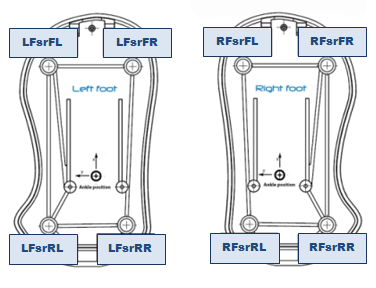
\includegraphics[scale=0.75]{pics/naosfeet.jpg}
	\label{fig:fsr_plot2}
    \caption{The force-sensitive resistors under Nao's feet (courtesy of
    Aldebaran Robotics)}
\end{figure}
There are different hardware implementations for the
Nao that can be used to figure out how stable it is in its current position. The one we use in this
reports are the force-sensitive foot sensors. There are four of these sensors on either foot
(as shown in Figure \ref{fig:fsr_plot2})
which give a constant reading of the current pressure on each of the sensors.

\subsection{The coordinate space}
\begin{figure}[htb]
	\centering
	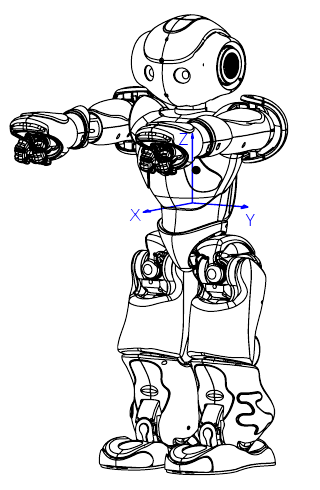
\includegraphics[scale=0.6]{pics/hardware_inertialunit.png}
	\label{fig:hardware}
    \caption{A schematic drawing of the Nao, showing his axis (courtesy of
    Aldebaran Robotics)}
\end{figure}

Figure \ref{fig:hardware} shows the way in which the coordinate system works that we
apply in our report. The x-axis point to the fron of the Nao, while the y-axis
points to the side and the z-axis upwards. All mentions of these axis in this
report will be around this same coordinate frame.



\section{Motivation for this project} 
While the Dutch Nao Team\cite{DNT2012} (the team that represents the Netherlands
in the Standard Platform League of the RoboCup) has achieved some degree of
success with simple keyframe motions, they are clearly not optimal; a lot of
time is wasted positioning the robot at just the right angle relative to kick
the ball towards the goal. Furthermore, if the ball gets moved after the kicking
motion has started, it is impossible for the robot to correct its kicking path.
These are all problems that can be reduced with a dynamically generated motion,
which is why we attempt to create one. 


\subsection{Stability in a match}
Since there is more than one player on
the field  chasing after the ball,
lots of interference can be expected from pushing Naos while trying to perform a kick. Due to the
instability of the Nao this results in falling down quite often, even more
so when there is no compensation for it when executing a motion. A dynamic
kick keeps track of how stable Naos current position is and compensates for
outside disturbances while kicking. 

\subsection{Harder kicks and better stability}
Being able to define when a kick is stable enough to execute we can make a
trade-off between how far the ball is kicked and the stableness of the
robot, resulting in harder kicks then when using keyframe motions.

\subsection{Helping the Dutch Nao Team}
 Working on this project will help the Dutch Nao Team in their competition. The
current keyframe motion used by DNT is very brittle. With our dynamic kick we
create a
more robust kick that can give our universities team a bigger chance of
winning in competitions. 
This integration makes this project a valuable activity in the long run, and not
just a one time experiment that would not be further developed.

\section{Methodology}
The task of kicking a ball requires a couple of things: We need to plan a path
for the foot to travel, then we need a way to calculate the joint angles
corresponding to the required position of the foot (inverse kinematics), and all
the while we have to make sure the robot doesn't fall over.

\subsection{Automatic balancing during the kicking motion}
The Nao should be balanced during its kick, regardless of the motion of the
kicking leg. For this a center of mass-based approach (\cite{Xu2010}) is used
along with a proportional
controller\footnote{http://www.societyofrobots.com/programming\_PID.shtml}.

\subsubsection{Center of mass and support polygon}
This balancing approach requires knowledge of 2 concepts; the \emph{center of mass},
and the \emph{support polygon}. The center of mass (\emph{CoM}) is the weighted average
location of the Nao's mass, while the support polygon is the location on the
floor over which the center of mass must be located to achieve stability. In the
case of a robot standing on the ground, the support polygon is the convex hull
of the feet touching the ground. Because the CoM is only used in conjuction with
a proportional controller (which only requires a single target point) and the
robot will only be balancing on one foot, the support polygon can be simplified
to be a single point slightly in front of the location of the support leg's ankle
joint.

The center of mass is defined as the sum of each component's
\emph{centroid} (its own center of mass) multiplied by its mass,
divided by the total weight (equation \ref{eq:CoM}). This of course
requires each centroid to be described in the same coordinate system.
\begin{align}
  \frac{\sum_i \vec{c}_i m_i} {m}        \label{eq:CoM}
\end{align}
In the Nao's documentation, each component's centroid is described relative to
its own coordinate system, and offsets are included to convert between adjacent
components’ coordinate systems. To handle this, we construct a chain of
transformations to walk through each component while calculating the center of
mass of the entire robot.

\subsubsection{The proportional controller}
The goal of the proportional controller (\emph{P-controller}) is to keep the
CoM as close as possible to the center of the support polygon at all times.
The CoM is calculated relative to the standing leg's ankle joint, and we define
the center of the support polygon to be ``about 3 cm in front of that''. Thus the
error-calculation becomes:
\begin{align}
  \begin{bmatrix} error_x \\ error_y \end{bmatrix} = \begin{bmatrix} 3 \\ 0 \end{bmatrix} - \vec{CoM_{xy}} 
\end{align}
The $z$-axis is ignored, because the height is irrelevant in this case (the CoM
balancer only accounts for gravity, not other phenomena such as momentum).

The proportional control equation with two arbitrary \emph{gain} parameters is
shown in (\ref{eq:pcontrolx}) and (\ref{eq:pcontroly}). The use of a different gain
parameter for the x- and y-directions allows compensation for the fact that the
Nao's feet (and really, feet in general) are rather elongated in the forward
direction, making them far more stable to forces along the $x$-axis as opposed to
the $y$-axis.
\begin{align}
  P_{out_{x}} = gain_x * error_x        \label{eq:pcontrolx} \\
  P_{out_{y}} = gain_y * error_y        \label{eq:pcontroly}
\end{align}
The value of $P_{out_{x}}$ is inverted when balancing on the left leg because of
the direction the joint rotates.

Actuation is achieved solely through the ankle's pitch and roll of the support
leg. The rotation angles are obtained by searching through the set
\begin{align*}
  \{ (\theta_{pitch}, \theta_{roll}) \mid \theta_{pitch} \in \{0, P_{out_{x}}\},
  \theta_{roll} \in \{0, P_{out_{y}}\} \}
\end{align*}
and selecting the pair of angles with the largest reduction in error. This
avoids situations where both components of the actuation interfere with
each other and actually make the robot more unstable. This approach is acceptably
fast when actuating two joints, but has the downside of having a complexity of
$\mathcal{O}(2^n)$ in amount of actuated joints.

\subsection{Using force-sensitive resistors to keep balance}

Although the CoM-based balancing allows for good convergence to a
stable position, it does not react to external influences.
Using the force-sensitive resistors under Nao's feet, these external influences can be measured and neutralized.
\begin{figure}[htb]
	\centering
	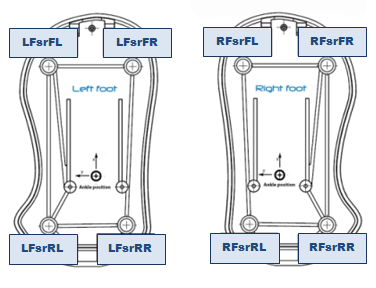
\includegraphics[scale=0.75]{pics/naosfeet.jpg}
	\label{fig:fsr_plot}
	\caption{The force-sensitive resistors}
\end{figure}\\
The foot of the support leg will be divided into four sections (Front, Left, Right and Back). 
\begin{itemize}
    \item $Front_t = (1-s) * Front_{t-1} + s * (LFsrFL + LFsrFR)$
    \item $Left_t = (1-s) * Left_{t-1} + s *(LFsrFL + LFsrRL)$
    \item $Right_t = (1-s) * Right_{t-1} + s *(LFsrFR + LFsrRR)$
    \item $Back_t = (1-s) * Back_{t-1} + s *(LFsrRL + LFsrRR)$ 
\end{itemize}
Where $s$ is the smoothing parameter and $t$ is the present time.

\subsubsection{Proportional-Derivative controller}

The Proportional-Derivative controller (PD-controller) is a special case of the
Proportional-Integral-Derivative controller (PID controller) where the integral
term (I) is not used.  The PD-controller has 2 terms, the proportional (P) and
the derivative (D) term. The response of each term can be tweaked using their own tweaking parameter, the proportional gain $K_p$ and the derivative gain $K_d$. \\
The proportional term is given by:
\[
P_{out}  = K_pe(t)
 \]
and the derivative term is given by:
\[
D_{out}  = K_d\frac{d}{dt}e(t)
\]
The hip pitch is used to compensate for the error in the $x$ direction ($Front$
and $Back$) while the hip roll compensates for the error in the $y$ direction
($Right$ and $Left$).
The angle offsets for the hip joints are calculated by
\begin{itemize}
    \item $e(t)_x = (Front_t - Back_t)$
    \item $e(t)_y = (Right_t - Left_t)$
    \item $P_{out} x = e(t)_xK_p$
    \item $P_{out} y = e(t)_yK_p$
    \item $D_{out} x = \frac{e(t)_x - e(t-1)_x}{timeTaken}K_d$
    \item $D_{out} y = \frac{e(t)_y - e(t-1)_y}{timeTaken}K_d$
    \item  $Offset$ $Hip$ $Pitch$ $= P_{out}x + D_{out}x$ 
    \item $Offset$ $Hip$ $Roll$ $=  P_{out}y + D_{out}y$ 
\end{itemize}
Where $timeTaken = time_t - time_{t-1}$(the time taken between the current and previous execution).

Using an error band allows for a range of stable points and therefore better
convergence. Without this range the robot would diverge and finally fall due to
oscillation. When the error is within this range it will be set to 0, this
allows the robot to converge to a stable position. Due to the robot's build the
forward and sideways stabilization act differently, different error bands are
needed for either side. The function of the proportional term becomes:
\[
  P_{out}x = \left\{ 
  \begin{array}{l l}
     e(t)_xK_p& \quad \text{if $e(t)_x < Thres_{min X}$ or $e(t)_x > Thres_{max X}$}\\ 
     0& \quad \text{Otherwise}\\
  \end{array} \right.
\]
\[
  P_{out}y = \left\{ 
  \begin{array}{l l}
      e(t)_yK_p& \quad \text{if $e(t)_y < Thres_{min Y}$ or $e(t)_y > Thres_{max Y}$}\\ 
     0& \quad \text{Otherwise}\\
  \end{array} \right.
\]
Where $Thres_{min}$ is the lower bound of the error band, $Thres_{max}$ is the upper bound
and $K_p$ is the  first tweak parameter of the PD-controller.\\
$Thres_{min X} = -Thres_{max X}$ and
$Thres_{min Y} = -Thres_{max Y}$.
\[
  D_{out}x = \left\{ 
  \begin{array}{l l}
      \frac{e(t)_x - e(t-1)_x}{timeTaken}K_d& \quad \text{if $e(t)_x < Thres_{min X}$  or $e(t)_x > Thres_{max X}$}\\ 
     0& \quad \text{Otherwise}\\
  \end{array} \right.
\]
\[
  D_{out}y = \left\{ 
  \begin{array}{l l}
     \frac{ e(t)_y - e(t-1)_y}{timeTaken}K_d& \quad \text{if $e(t)_y < Thres_{min Y}$ or $e(t)_y > Thres_{max Y}$}\\ 
     0& \quad \text{Otherwise}\\
  \end{array} \right.
\]

\subsubsection{Sampling Rate Issues}

Using the balancer as it is now requires different parameters for every sampling rate.
Since the sampling rate is determent by the available CPU power, a fix is needed that will added the sampling rate in the calculation.
Doing this allows the same parameters to be used regardless of the background processes or CPU type.
The follow fix is applied:
\begin{itemize}
	\item $Offset$ $Hip$ $Pitch$ $= (P_{out}x + D_{out}x) * timeTaken $ 
	\item $Offset$ $Hip$ $Roll$ $=  (P_{out}y + D_{out}y) * timeTaken$ 
\end{itemize}
With this fix the angle offsets will be relative to $timeTaken$, giving a bigger offset when the time between the executions is larger and vice versa. This gives us a timing-independent compensation architecture which adapts to the available CPU power.

\subsubsection{The setup error}

As the script runs the first measurements of $timeTaken$ are relative big in some cases even a factor 100 from the normal value.
This big value will change the angles in such a way the robot will overshoot and possibly even fall.
Therefore disregarding these values will be necessary, adding a low-pass filter
to $\Delta timeTaken$ allows finding these measurements. When the threshold of the low-pass filter has been exceeded the angle offsets will be set to 0, ignoring the large values.
\[
  Offset hip pitch = \left\{ 
  \begin{array}{l l}
     (P_{out}x + D_{out}x)  * timeTaken& \quad \text{if $\Delta timeTaken < Thres_{low-pass}$}\\ 
    0 & \quad \text{Otherwise}\\
  \end{array} \right.
\]

\[
  Offset hip roll = \left\{ 
  \begin{array}{l l}
     (P_{out}y + D_{out}y)  * timeTaken& \quad \text{if $\Delta timeTaken < Thres_{low-pass}$}\\ 
    0 & \quad \text{Otherwise}\\
  \end{array} \right.
\]
Where $Thres_{low-pass}$ is the threshold value for the low-pass filter.

\subsection{The kinematics problem}
\label{sec:ik}
We want to be able to specify a location for the foot, then have the foot
automatically move there, which means that the we'll need to be able calculate
the required joint angles. This is known as \emph{inverse kinematics}. There is
a number of potential solutions to this problem, for example: 
\begin{itemize}
\item analytically solve the inverse kinematics chain using goniometry (as done by \cite{Graf2009})
\item use an iterative algorithm to approach the desired location over a number
  of iterations (\cite{Buss2009})
\end{itemize}

We wound up going with an iterative, Jacobian-based solution as decribed by
\cite{Meredith2004} and \cite{Buss2009}. To see a short summary of other
experimentations, see appendix \ref{A}.

\subsubsection{Problem specification and terminology}
Let:
\begin{itemize}
    \item $\theta$ be a $1 \times n$ vector describing the angles of $n$ joints
        ($\theta = \bvect{\theta_1 & \dots & \theta_n}^T$)
    \item $\vec{t}$ the vector containing the goal position for each end effector
    \item $\vec{s}$ the vector of the end effectors' current positions
\end{itemize}

$\vec{t}$ and $\vec{s}$ are both of size $1 \times f$ where $f$ is the
desired amount of degrees of freedom in the end effectors (generally 3
if you only care about the spatial location, or 6 if you take the
rotation into account too).  Thus, if you have $k$ end effectors and 3
degrees of freedom in your position:

\begin{align*}
    \vec{t} &= \bvect{t_1, &\dots, &t_k}^T \\
    \vec{s} &= \bvect{s_1, &\dots, &s_k}^T
\end{align*}
where
\begin{align*}
    t_i &= \bvect{t_{i_{x}}, &t_{i_{y}}, &t_{i_{z}}}^T \\
    s_i &= \bvect{s_{i_{x}}, &s_{i_{y}}, &s_{i_{z}}}^T
\end{align*}

Viewing the end effectors locations as a function of the joint angles,
we want to find values for $\theta$ such that $\vec{t} =
\vec{s}(\theta)$. One way to do this is by taking a linear
approximation of the function with respect to the joint angles, and
slightly adjusting the angles to get closer to the solution.  Over a
number of iterations, the end effectors will hopefully converge to the
desired position.  This linear approximation is done using the
Jacobian matrix $J$, defined as:
\begin{align}
  J(\theta)_{i, j} &= \frac{\partial s_i}{\partial \theta_j} \\
  \frac{\partial s_i}{\partial \theta_j} &= v_j \times (s_i - p_j)    \label{eq:fillJ}
\end{align}
In the case of a rotational joint (as is the case with every joint on
the Nao robot), the the entries of the Jacobian are given by
(\ref{eq:fillJ}), where $v_j$ is a unit vector describing the axis of
rotation of the joint belonging to $\theta_j$ and $p_j$ is the
location of that joint in space.

Using the Jacobian matrix, the change in end effector locations
corresponding with a certain change in joints angles can be described
as:
\begin{align*}
  \Delta \vec{s} \approx J \Delta \theta
\end{align*}
$\Delta \vec{s}$ should be as close as possible to the error $\vec{e}
= \vec{t} - \vec{s}$, which means that the equation
we're looking for is:
\begin{align*}
  \Delta \theta = J^{-1} \vec{e}
\end{align*}

Since the Jacobian will generally not be invertable, its inverse will
have to be approximated. Some methods of approximation include the
Jacobian transpose method, the Moore-Penrose pseudo-inverse, and the
Levenberg-Marquardt damped least squares method (see \cite{Buss2009}).

\subsubsection{The algorithm}
We opted to go for a 3-dimensional positioning, without regards for the rotation
of the end-effector (see section \ref{sec:kick} for motivation). Because the
ankle joint is taken as end-effector, the ankle itself has no influence on the
location. This leaves us with 4 joints; the pitch, roll and yaw of the hip,
along with the knee's pitch.

Because the Jacobian only gives a linear approximation, the joints
tend to behave erratically when a target location is far away. This is
counteracted by moving the target closer if the distance exceeds a
certain threshold. This is done according to (\ref{eq:clampmag}).
\begin{align}
  \vec{e} = \begin{cases}
    \vec{t} - \vec{s} & \text{if } ||\vec{t} - \vec{s}|| < D_{max} \\
    D_{max} \frac{\vec{t} - \vec{s}}{||\vec{t} - \vec{s}||}
  \end{cases}      \label{eq:clampmag}
\end{align}

Pseudocode for the algorithm can be seen in algorithm \ref{code:ik}.

\begin{algorithm}
  \begin{algorithmic}
    \Function{inverse\_kinematics}{$target$, $\lambda$, $max\_iter$, $D_{max}$, $threshold$}
      \State $best\_error = \infty$
      \State $best\_\theta = nil$
      \State $\theta \gets$ the current body angles
      \While{$n\_iter < max\_iter$}
        \State $\vec{s} \gets $the current end effector position
        \State $\vec{e} \gets target - \vec{s}$
        \State $error \gets ||\vec{e}||$

        \If{$error < best\_error$}
          \State $best\_error \gets error$
          \State $best\_\theta \gets \theta$
        \EndIf
        \If{$best\_error < threshold$}
          \State \Return $best\_\theta$
        \Else
          \State $J \gets get\_jacobian(\theta)$
          \If{$||\vec{e}|| > D_{max}$}
            \State $\vec{e} \gets D_{max} \frac{\vec{e}}{||\vec{e}||}$
          \EndIf
          \State $J^{-1} \gets J^T (J J^T)^{-1} + \lambda^2 I(3)$
          \Comment{I(3) is the $ 3\times 3$ identity matrix}
          \State $d\theta \gets J^{-1} * \vec{e}$
          \State $\theta \gets \theta + d\theta$
        \EndIf
      \EndWhile
      \State \Return $best\_\theta$
    \EndFunction
  \end{algorithmic}
  \caption{The inverse kinematics solution}
  \label{code:ik}
\end{algorithm}

When updating the joint angles ($\theta$), take care to restrict them to their
actual range to avoid a solution with impossible angles.

\subsection{The Kick}
\label{sec:kick}
With the solutions to the previous aspects of the dynamic kick constructed, 
we can start to calculate the optimal kicking trajectory. This kick is composed
of different stages, loosely based on the approach of \cite{Xu2010}. 
\begin{itemize}
    \item Initial pose
    \item Retraction point
    \item Contact point
\end{itemize}

For all these stages we assume we have knowledge about the coordinates of the
ball in some coordinate system relative to the Nao or a fixed point in space,
the size of the ball to hit and which way we want to kick the ball.

\subsubsection{Initial pose}
The first stage is the initial pose. The Nao positions its center of mass on
top of its standing leg. This is done by setting the Nao in NormalPose (a
keyframe motion made by the Dutch Nao Team) and
turning on the CoM-balancer.

\subsubsection{Contact point}
The contact point is the point on the ball that has to be hit by the Nao to
move it in the desired direction. \cite{Xu2010} uses the following
calculation to find this, which seems to work exactly as we would like:
\begin{align*}
    \vec{c} - ( \vec{e} * r )
\end{align*}
where $\vec{c}$ is the location of the center of mass of the ball, $r$ is the
ball radius (in the case of the SPL balls this is 33.42 mm) and $\vec{e}$ is the
force destination (the direction of where we want the ball to end up in
coordinates). 


\subsubsection{Retraction point}
After the initial pose the Nao calculates its optimal retraction point. This
is the rearmost point from which the kick commences, and has two criteria that
should be satisfied to be considered a good starting position:
\begin{itemize}
    \item The retraction point should be far away from the ball (to make the
        kick as hard as possible)
    \item The retraction point should be accurate 
\end{itemize}
To meet both criteria as good as possible there should be a trade off between
the two.

Firstly, to determine the point between the ball and a possible retraction point
we use the following calculation: 

\begin{align}
    d_r = \vec{e}^{x} * || \vec{p}^{x} -\vec{p}_{c}^{x}|| + \vec{e}^y *
||\vec{p}^{y} - \vec{p}_{c}^y|| +  ||
\vec{p}^z - \vec{p}_{c}^z|| * 0.3
\label{eq:distance}
\end{align}
Where $\vec{p_c}$ is the contact point where the ball should be hit,
$\vec{p}$ is a possible retraction point, $\vec{e}$ is the unit vector pointing
to the desired desination and $\vec{d_r}$ the distance between both
points. The importance of the $x$ and $y$ distance between the contact point and a possible
retraction point relies on how much of the unit vector points to that direction.
The $z$ is held artificially high so that the leg will never be stretched to the
ground.

\begin{figure}
  \resizebox{\textwidth}{!} {
    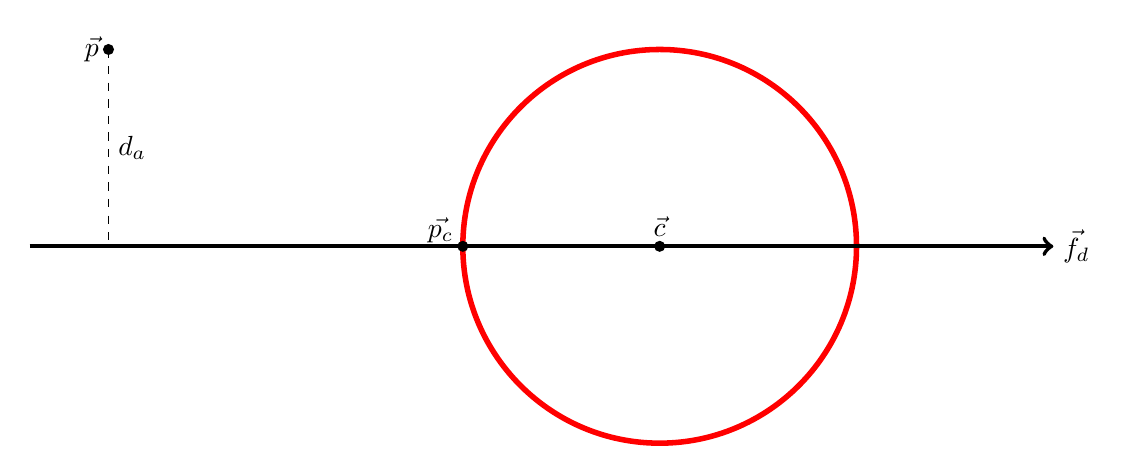
\begin{tikzpicture}
        \coordinate [label=left:$\vec{p_c}$] (A) at (-2.5,0.2);
        \coordinate [label=right:$\vec{f_d}$] (B) at (5, 0 );
        \coordinate [label=right:$d_a$] (F) at (-7, 1.25);
        \coordinate [label=above:$\vec{c}$](C) at (0,0);
        \coordinate (D) at (-2.5, 0);
        \coordinate [label=left:$\vec{p}$] (E) at (-7, 2.5);
        \draw[line width = 2][color = red] (0,0) circle (2.5cm);
        \draw [style = thick][line width = 1.5][->](-8, 0) -- (B);
        \draw[dashed] (E) -- (-7,0);
        \foreach \point in {C,D,E}
        \fill [black,opacity=1] (\point) circle (2pt);
    \end{tikzpicture}
    }
    \caption{Visualisation of the accuracy problem. \small{the contact point
            ($\vec{p_c}$) and the preferable force direction ($\vec{f_d}$) form a line
    in 3D space. A possible retraction point $\vec{p}$ can be somewhere around
    this line. To find its accuracy the distance $d_a$ should be solved. Note that
    this only concerns the x and y direction as the z dimension does not
    influence the accuracy. $\vec{c}$ denotes the center of mass
    location on the ball and is only shown for clarification.}}
    \label{fig:accuracy}
\end{figure}    

Finding the accuracy of a given retraction point is less straightforward. This
problem can be seen as the closeness of a given point to the line, where the
point consists of a possible retraction point and the line consits of the
contact point and the destination point. See Figure \ref{fig:accuracy} for a
visualisation of the problem. This idea makes for a basic linear algebra\footnote{The intuition behind this calculation can be found on http://mathworld.wolfram.com/Point-LineDistance3-Dimensional.html }
problem that needs to be resolved.
\begin{align*}
    d_a = \frac{||(\vec{p}^{xy} -\vec{p_c}^{xy}) \times (\vec{p}^{xy} -
    \vec{f_d}^{xy})||}{\|\vec{f_d}^{xy}- \vec{p_c}^{xy}\|}
\end{align*}

The distance to the line is only important in the $xy$ direction, but a cross
product can only be taken in 3D so this is solved by taking the $xy$
values from the original points in space but adding a 0 value in the z
direction.
Now that we have a way to calculate both the distance to the contact point and
the accuracy towards the force direction, we are able to make a balanced
decision towards what a good retraction point is.

\begin{align}
    \vec{p} = 1-\delta * d_r + \delta * \frac{100}{d_a}
\label{eq:delta}
\end{align}

We take the multiplicative inverse of $d_a$ so that the value gets bigger when the
retraction point is close to the line and rescale it by multiplying it with 100 to
make the value $d_r$ and $d_a$ more in the same range. The value $\delta$  could
be experimented with to find the optimal result.Accuracy is more important than a big distance between ball and
retraction point, something that will become evident in the results section.

All possible positions $\vec{p}$ should be considered to solve this equation. To
determine what is possible the Nao is set in different positions and using a
forward kinematics chain the end effector of each leg where the origin is the
supporting foot can be retrieved. This way roughly all possible positions are set and can be
looped through to find the point that maximizes above equation. By also
retrieving the location of the standing leg we make sure that there is
no overlap in the reachable space and the position of the other leg.

\section{Experiments and Results}

\subsection{Using force sensitive resistors for balancing}
\begin{figure}[htbp]
  \centering
  \makebox[\textwidth] {
    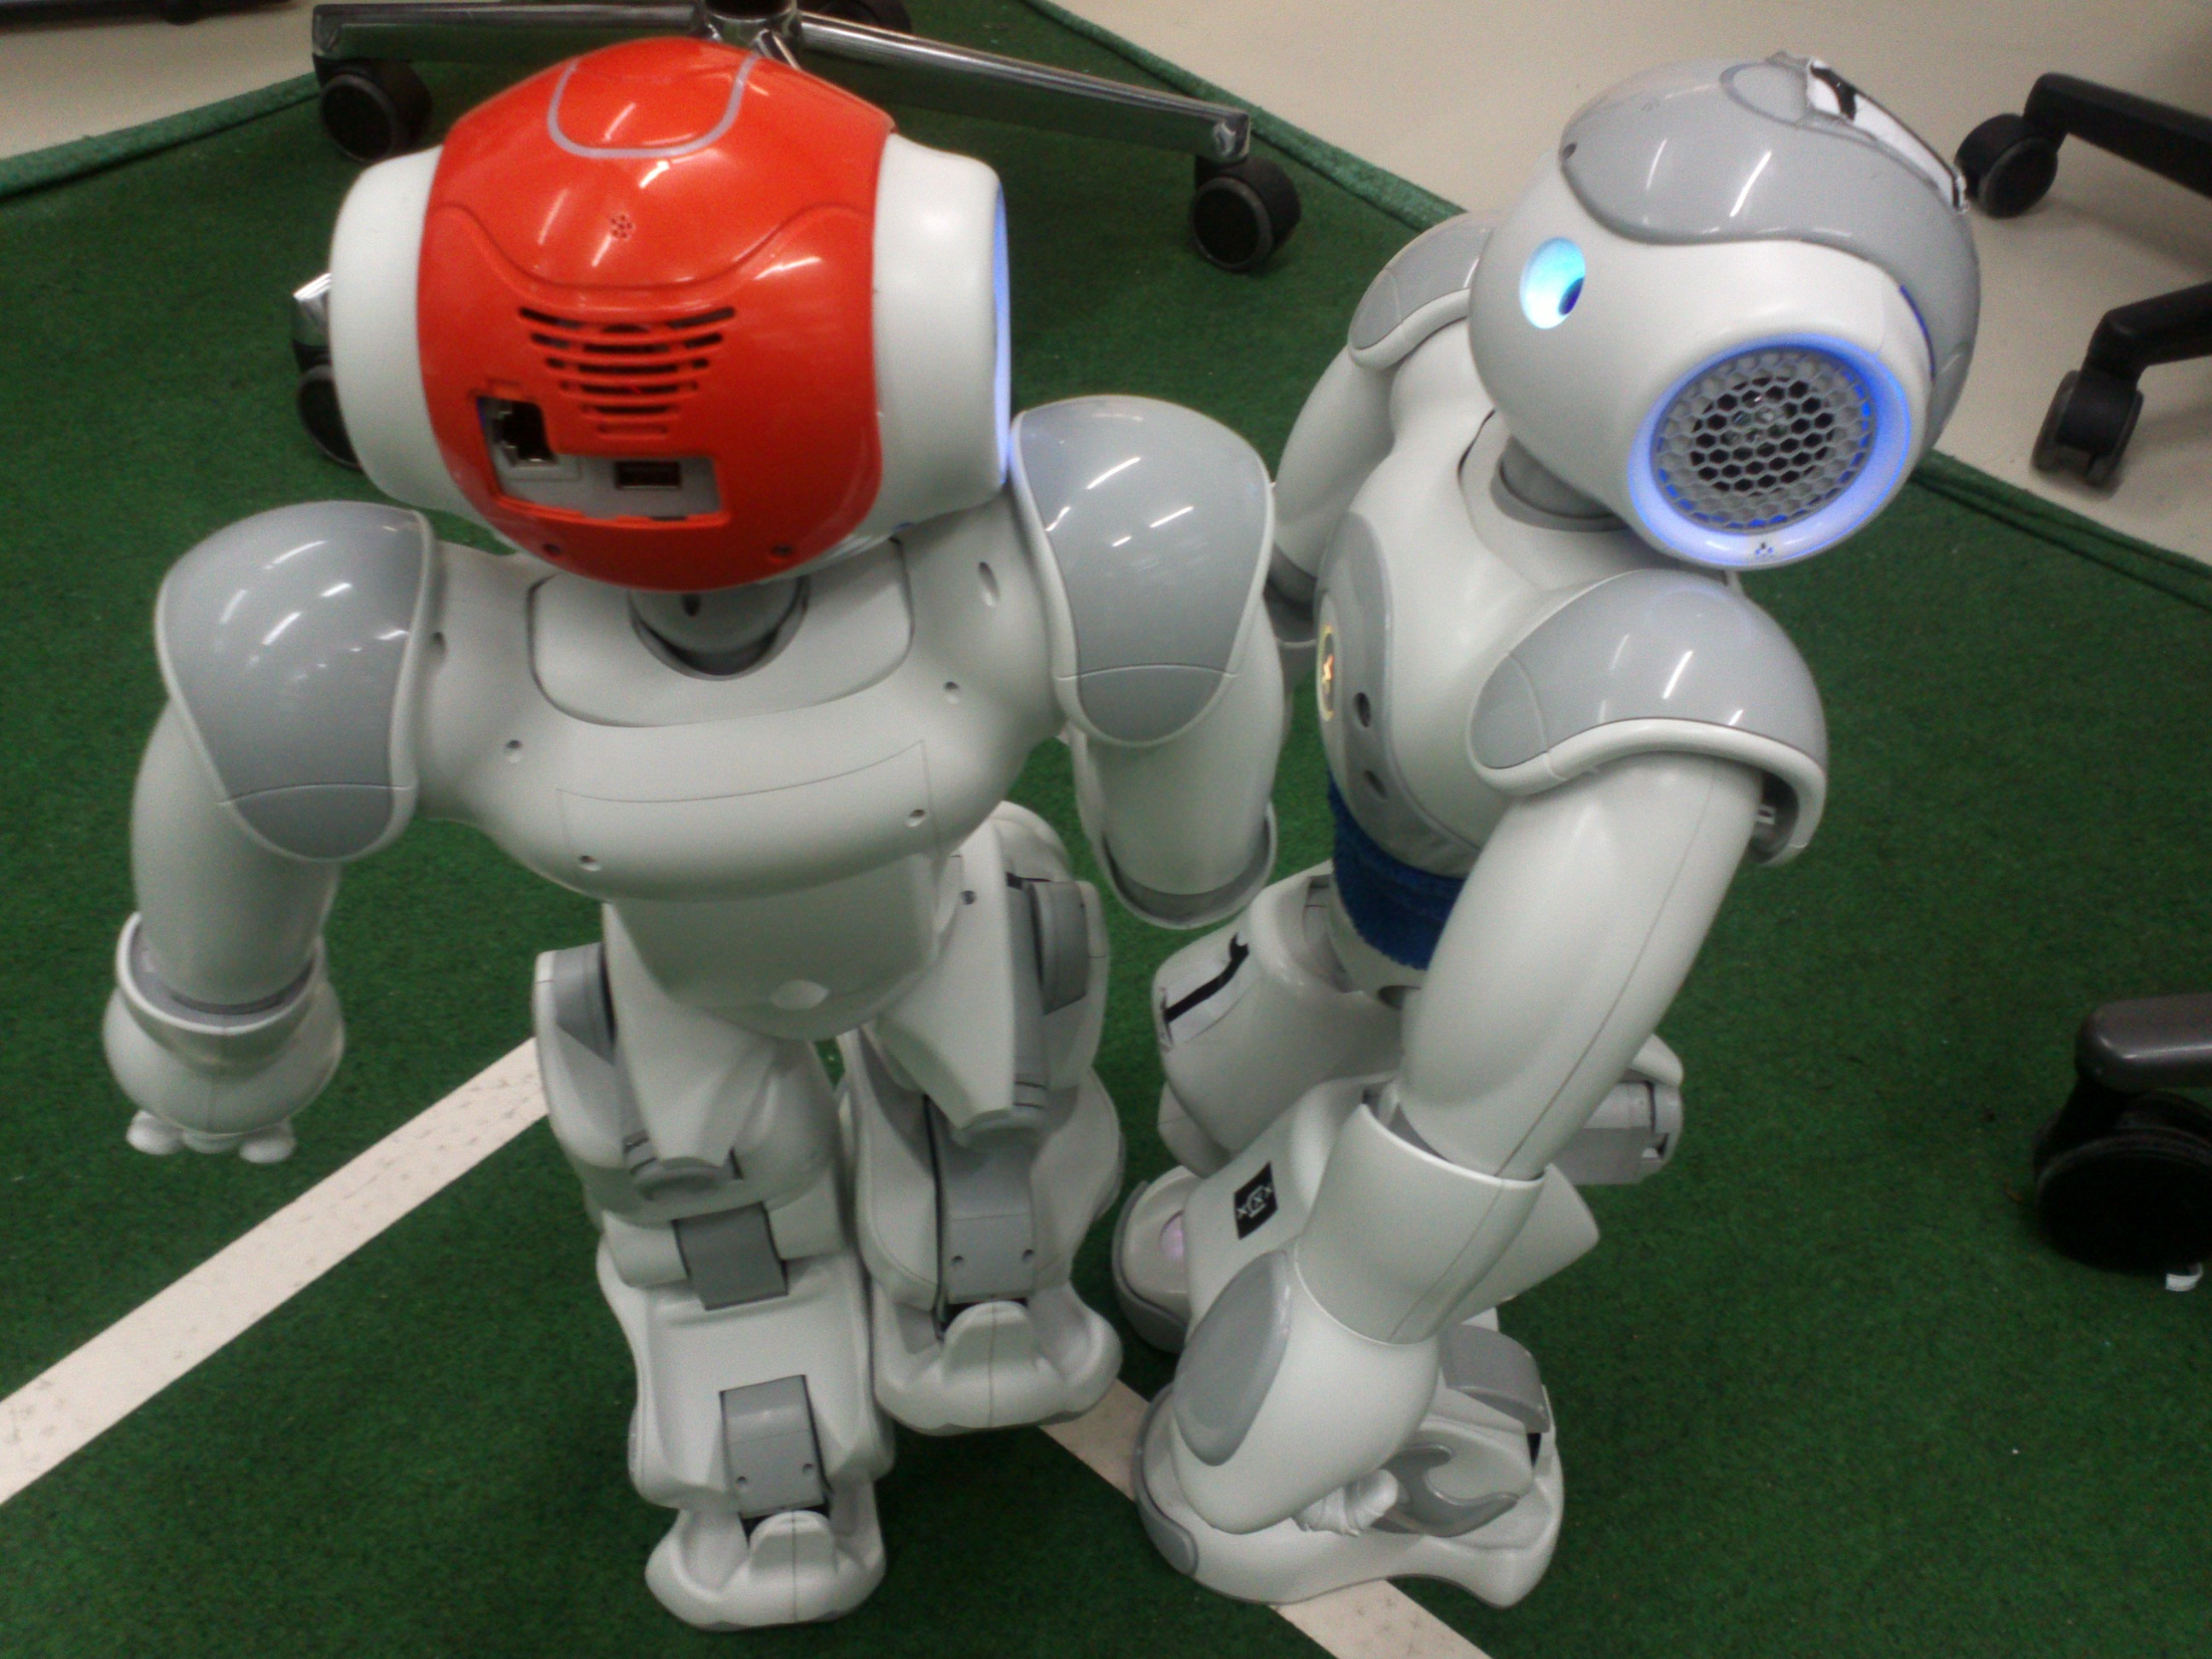
\includegraphics[scale = 0.1]{pics/nao_pushing_side}
  }
  \caption{Nao (right) pushing the other Nao (left) in the sideways (y) direction}
  \label{fig:pushing}
\end{figure}
\begin{figure}[htbp]
  \centering
  \makebox[\textwidth] {
    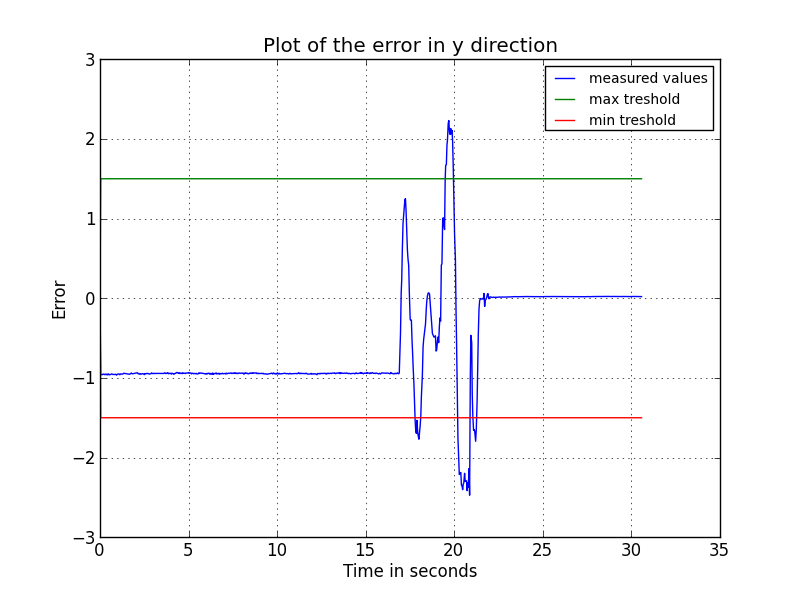
\includegraphics[scale = 0.7]{pics/y_without_balance}
  }
  \caption{With the balancer turned off (The Nao falls at 22 seconds)}
  \label{fig:pushing1}
\end{figure}
\begin{figure}[htbp]
  \centering
  \makebox[\textwidth] {
    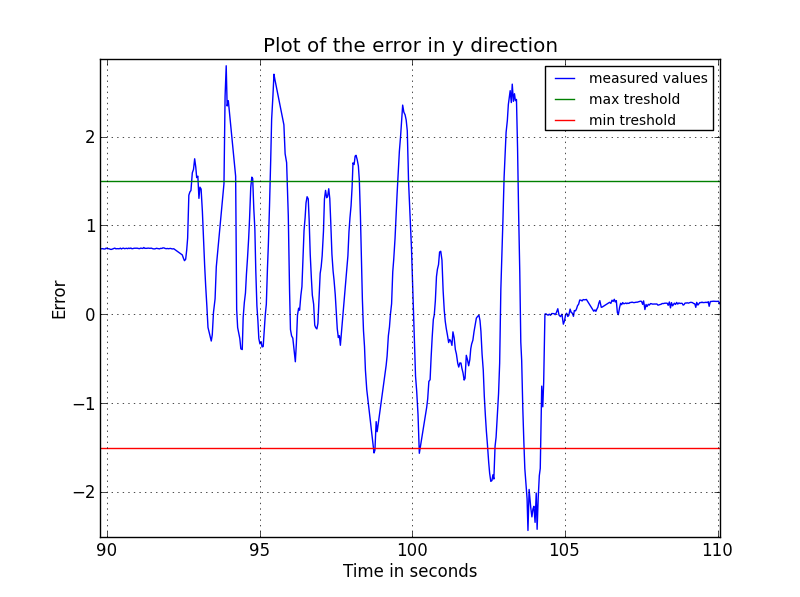
\includegraphics[scale = 0.6]{pics/y_with_balance}
  }
  \caption{With the balancer turned on (The Nao falls at 104 seconds)}
  \label{fig:pushing2}
\end{figure}
Since balancing in the $y$ direction is the biggest challenge to stabilize we used another Nao to push the balancing Nao in this direction (see  Figure \ref{fig:pushing}).
We ran the script twice, one time with the balancer on and the second time where the offsets of the angles where forced to 0  (keeping the plotting function but killing the balance system)\\\\
As seen in the plots (Figure \ref{fig:pushing1} and Figure \ref{fig:pushing2}), using the balancer helps to stay up longer (twice as long) but still can't fully handle the external influences from the pushing Nao.
The problem is that there aren't many stable poses in the sideways direction and even a small change will have a relative large influence on the sensor data.
Due to this the sideways balancing tends to overshoot and then start to oscillate.
Taking a low $K_p$ and $K_d$ values gives a long settling time but minimizes the overshoot.  
The system now converges relative slow to a stable position but is still able to negate external influences, providing a more stable and reliable balancer. 
\FloatBarrier
\subsection{Inverse kinematics}
\FloatBarrier
Since our inverse kinematics solution relies on two parameters
($\lambda$ and $D_{max}$, see section \ref{sec:ik}), some testing needs to be
done to optimize these. For testing, 3 reasonable target positions were chosen,
where the parameters were chosen from the set $\{\lambda, D_{max} \mid \lambda \in
  (0.1, 0.25, 0.5, 1, 5), D_{max} \in (10, 20, 30, 40, 50)\}$. The results can be
seen in figures \ref{fig:ik_plot1}, \ref{fig:ik_plot2} and \ref{fig:ik_plot3}.
The error in the plots is defined as $|| \vec{t} - \vec{s} ||$. Due to the large
number of colored squiggly lines, each plot has been restricted to only
parameter combinations which converged relatively quickly to aid in readability.

\begin{figure}[htbp]
  \centering
  \makebox[\textwidth] {
    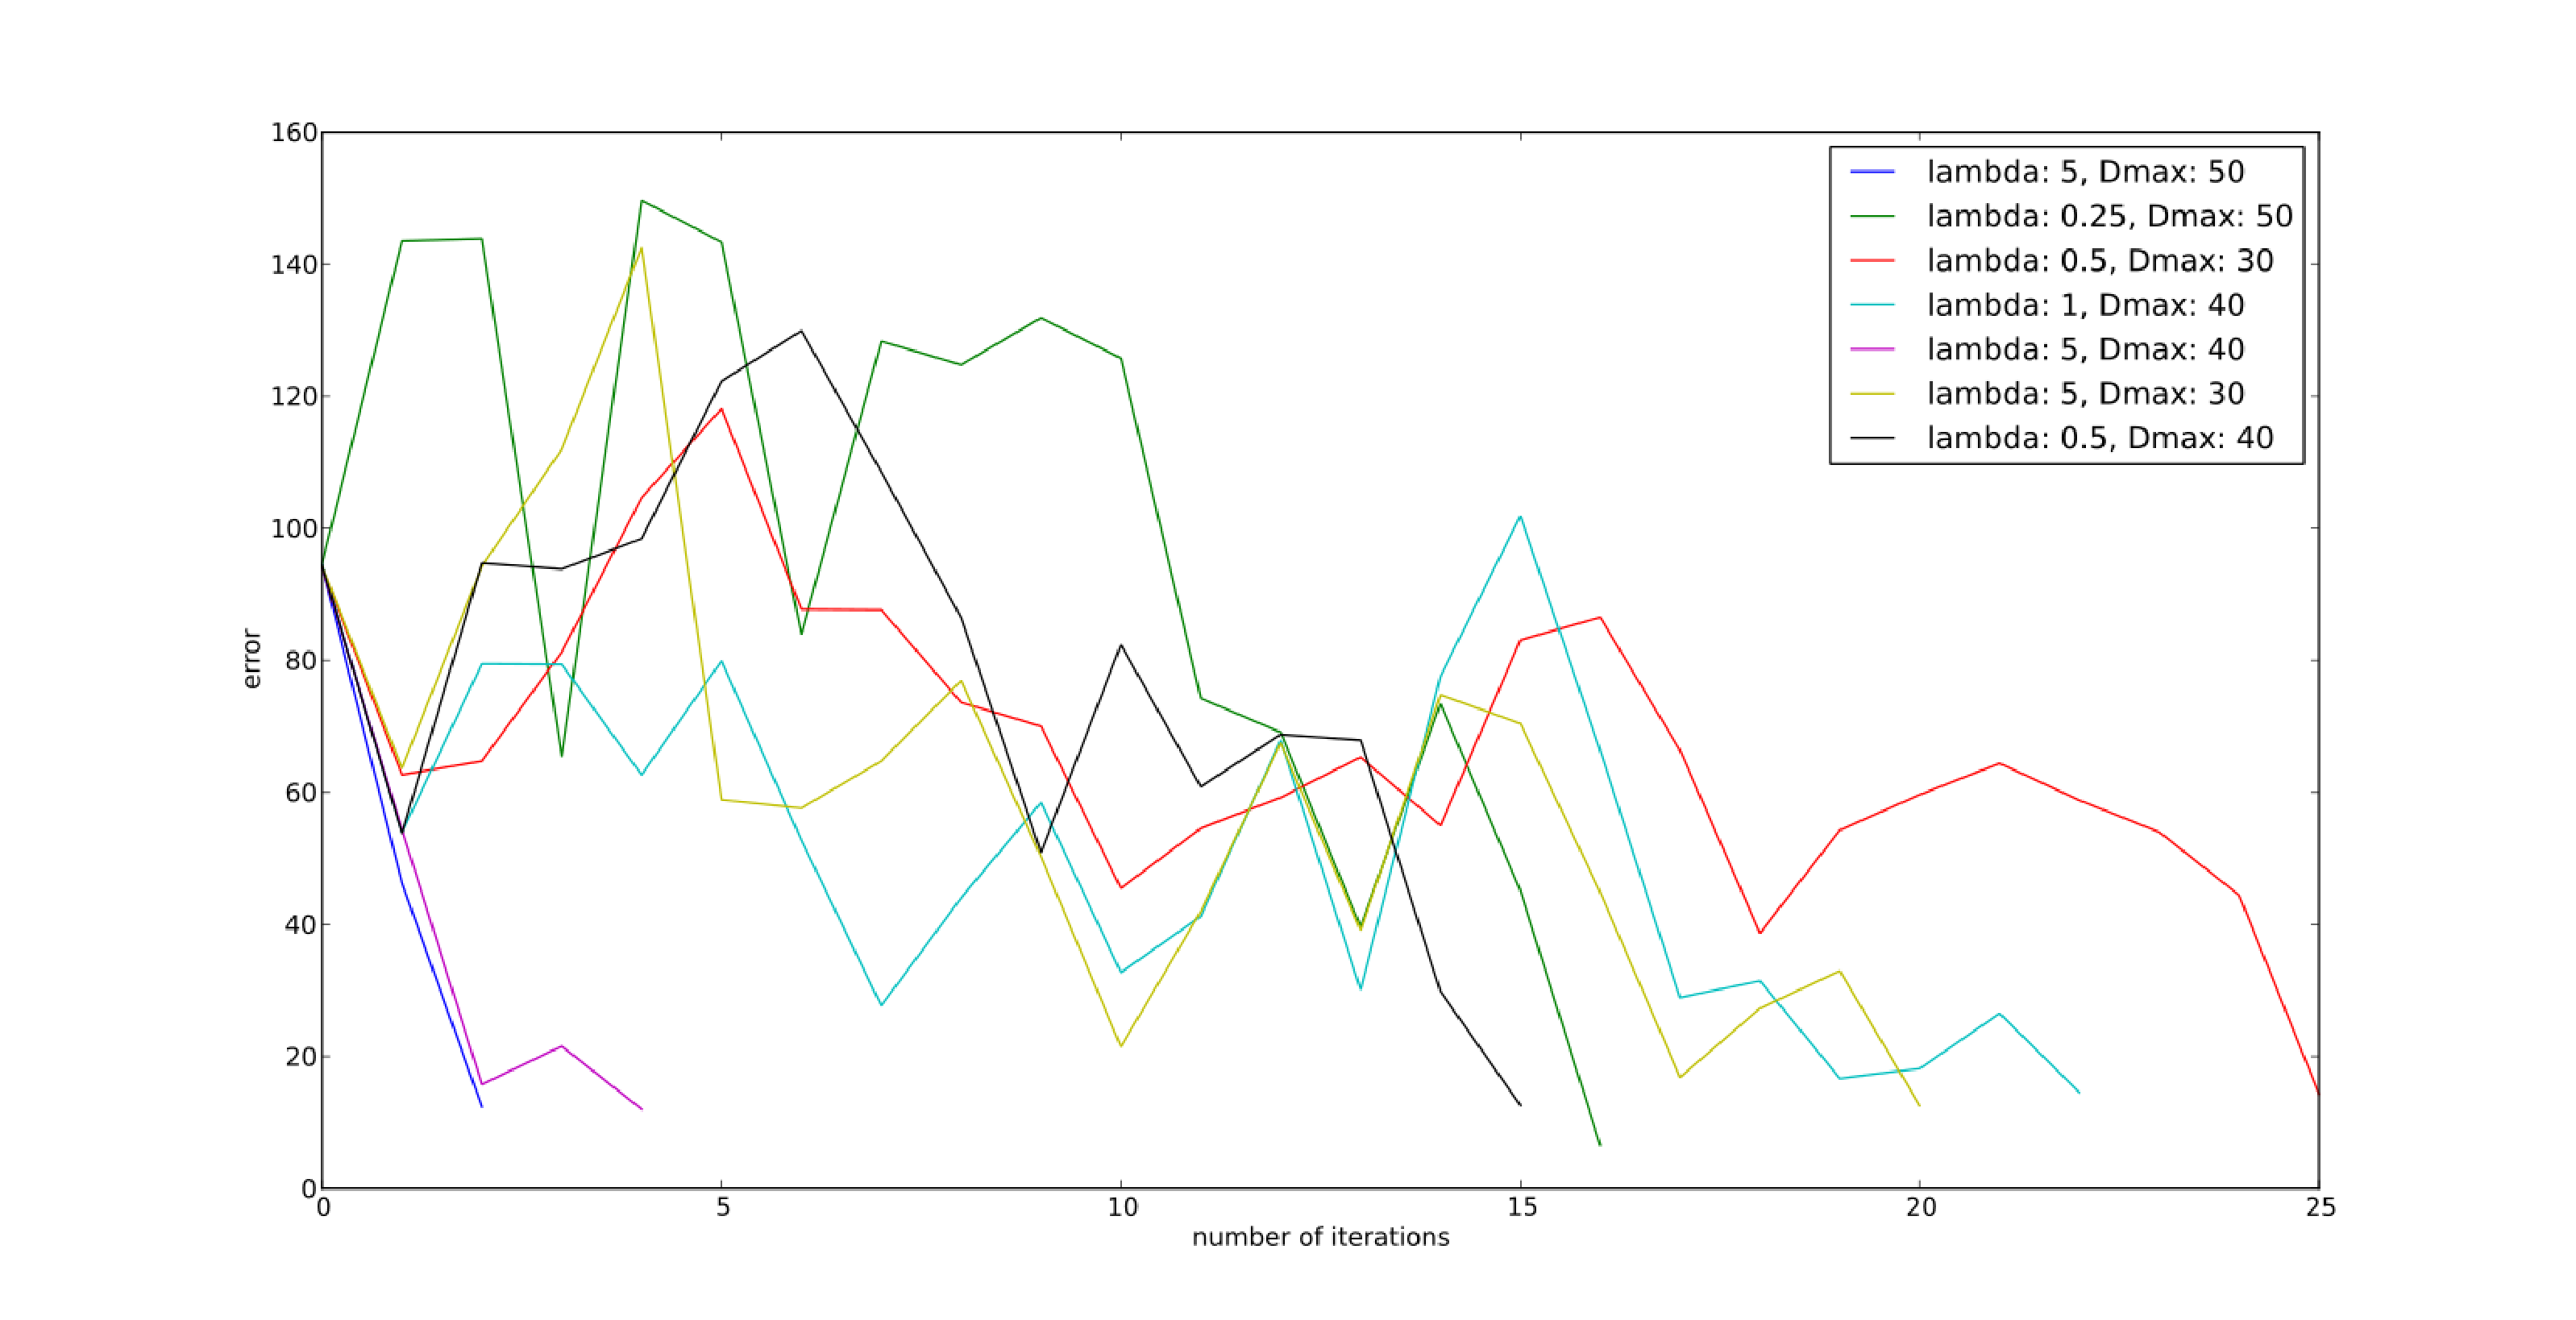
\includegraphics[width=1.3\textwidth]{pics/ik_1.pdf}
  }
  \caption{The first position, with the positional error set out against
         the time.}
  \label{fig:ik_plot1}
\end{figure}

\begin{figure}[htbp]
  \centering
  \makebox[\textwidth] {
    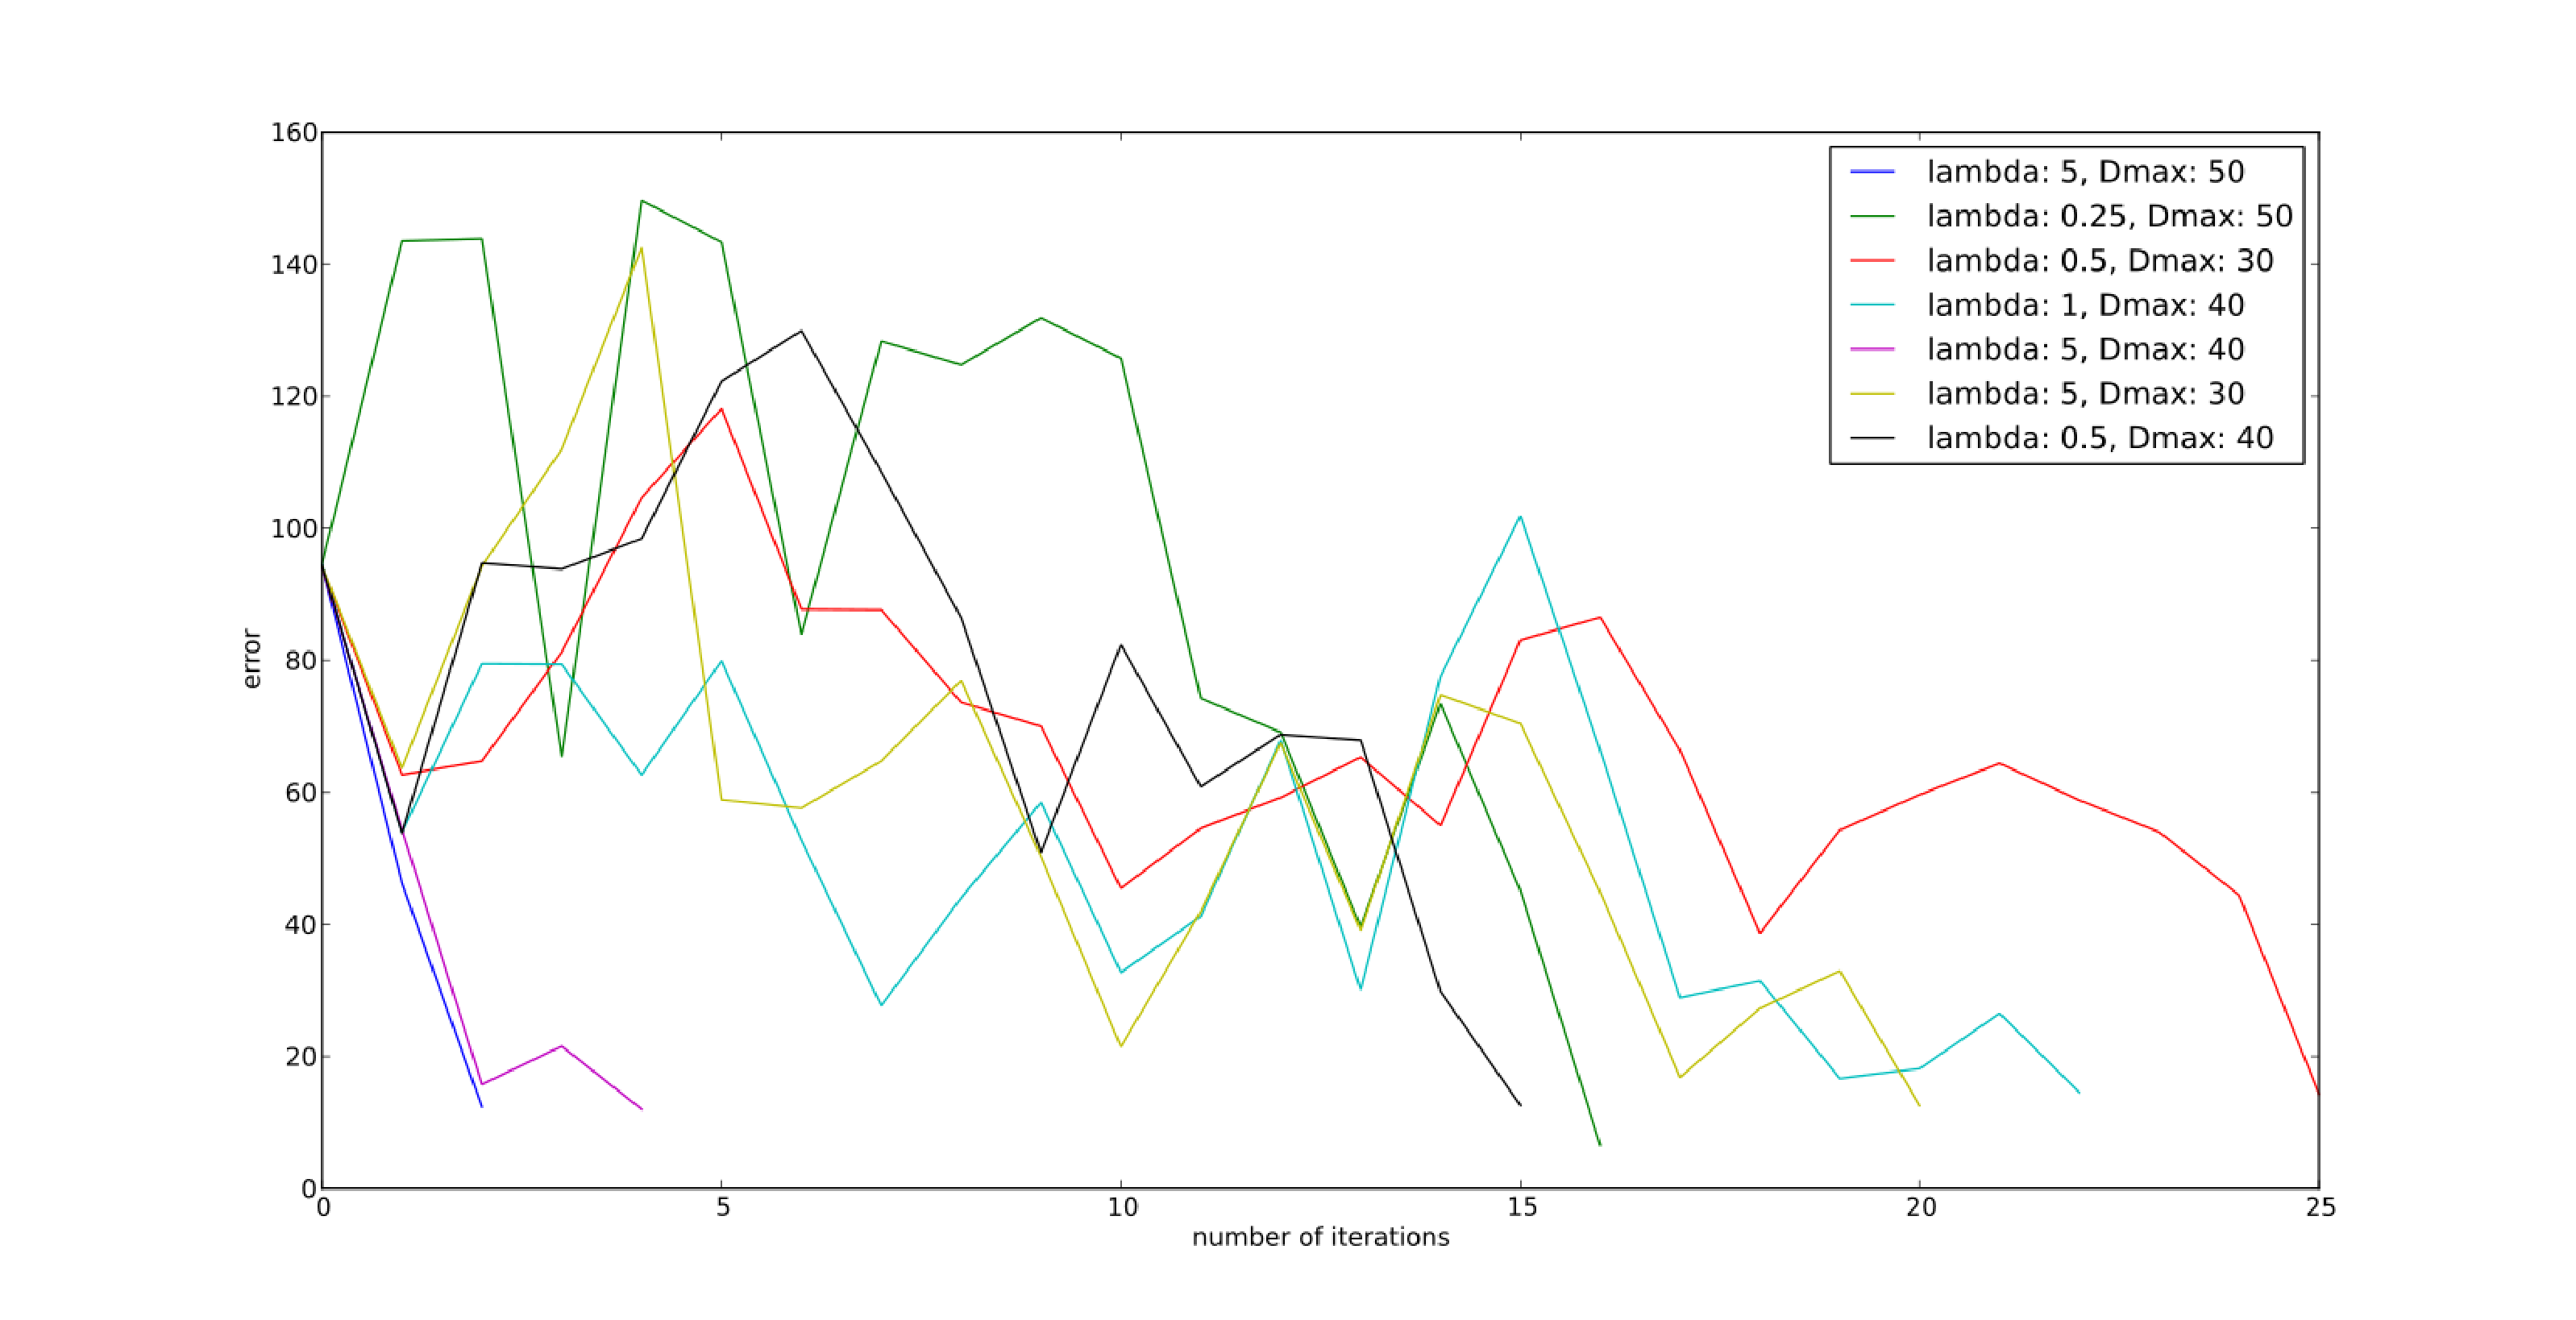
\includegraphics[width=1.3\textwidth]{pics/ik_1.pdf}
  }
  \caption{The second position, with the positional error set out against
         the time.}
  \label{fig:ik_plot2}
\end{figure}

\begin{figure}[htbp]
  \centering
  \makebox[\textwidth] {
    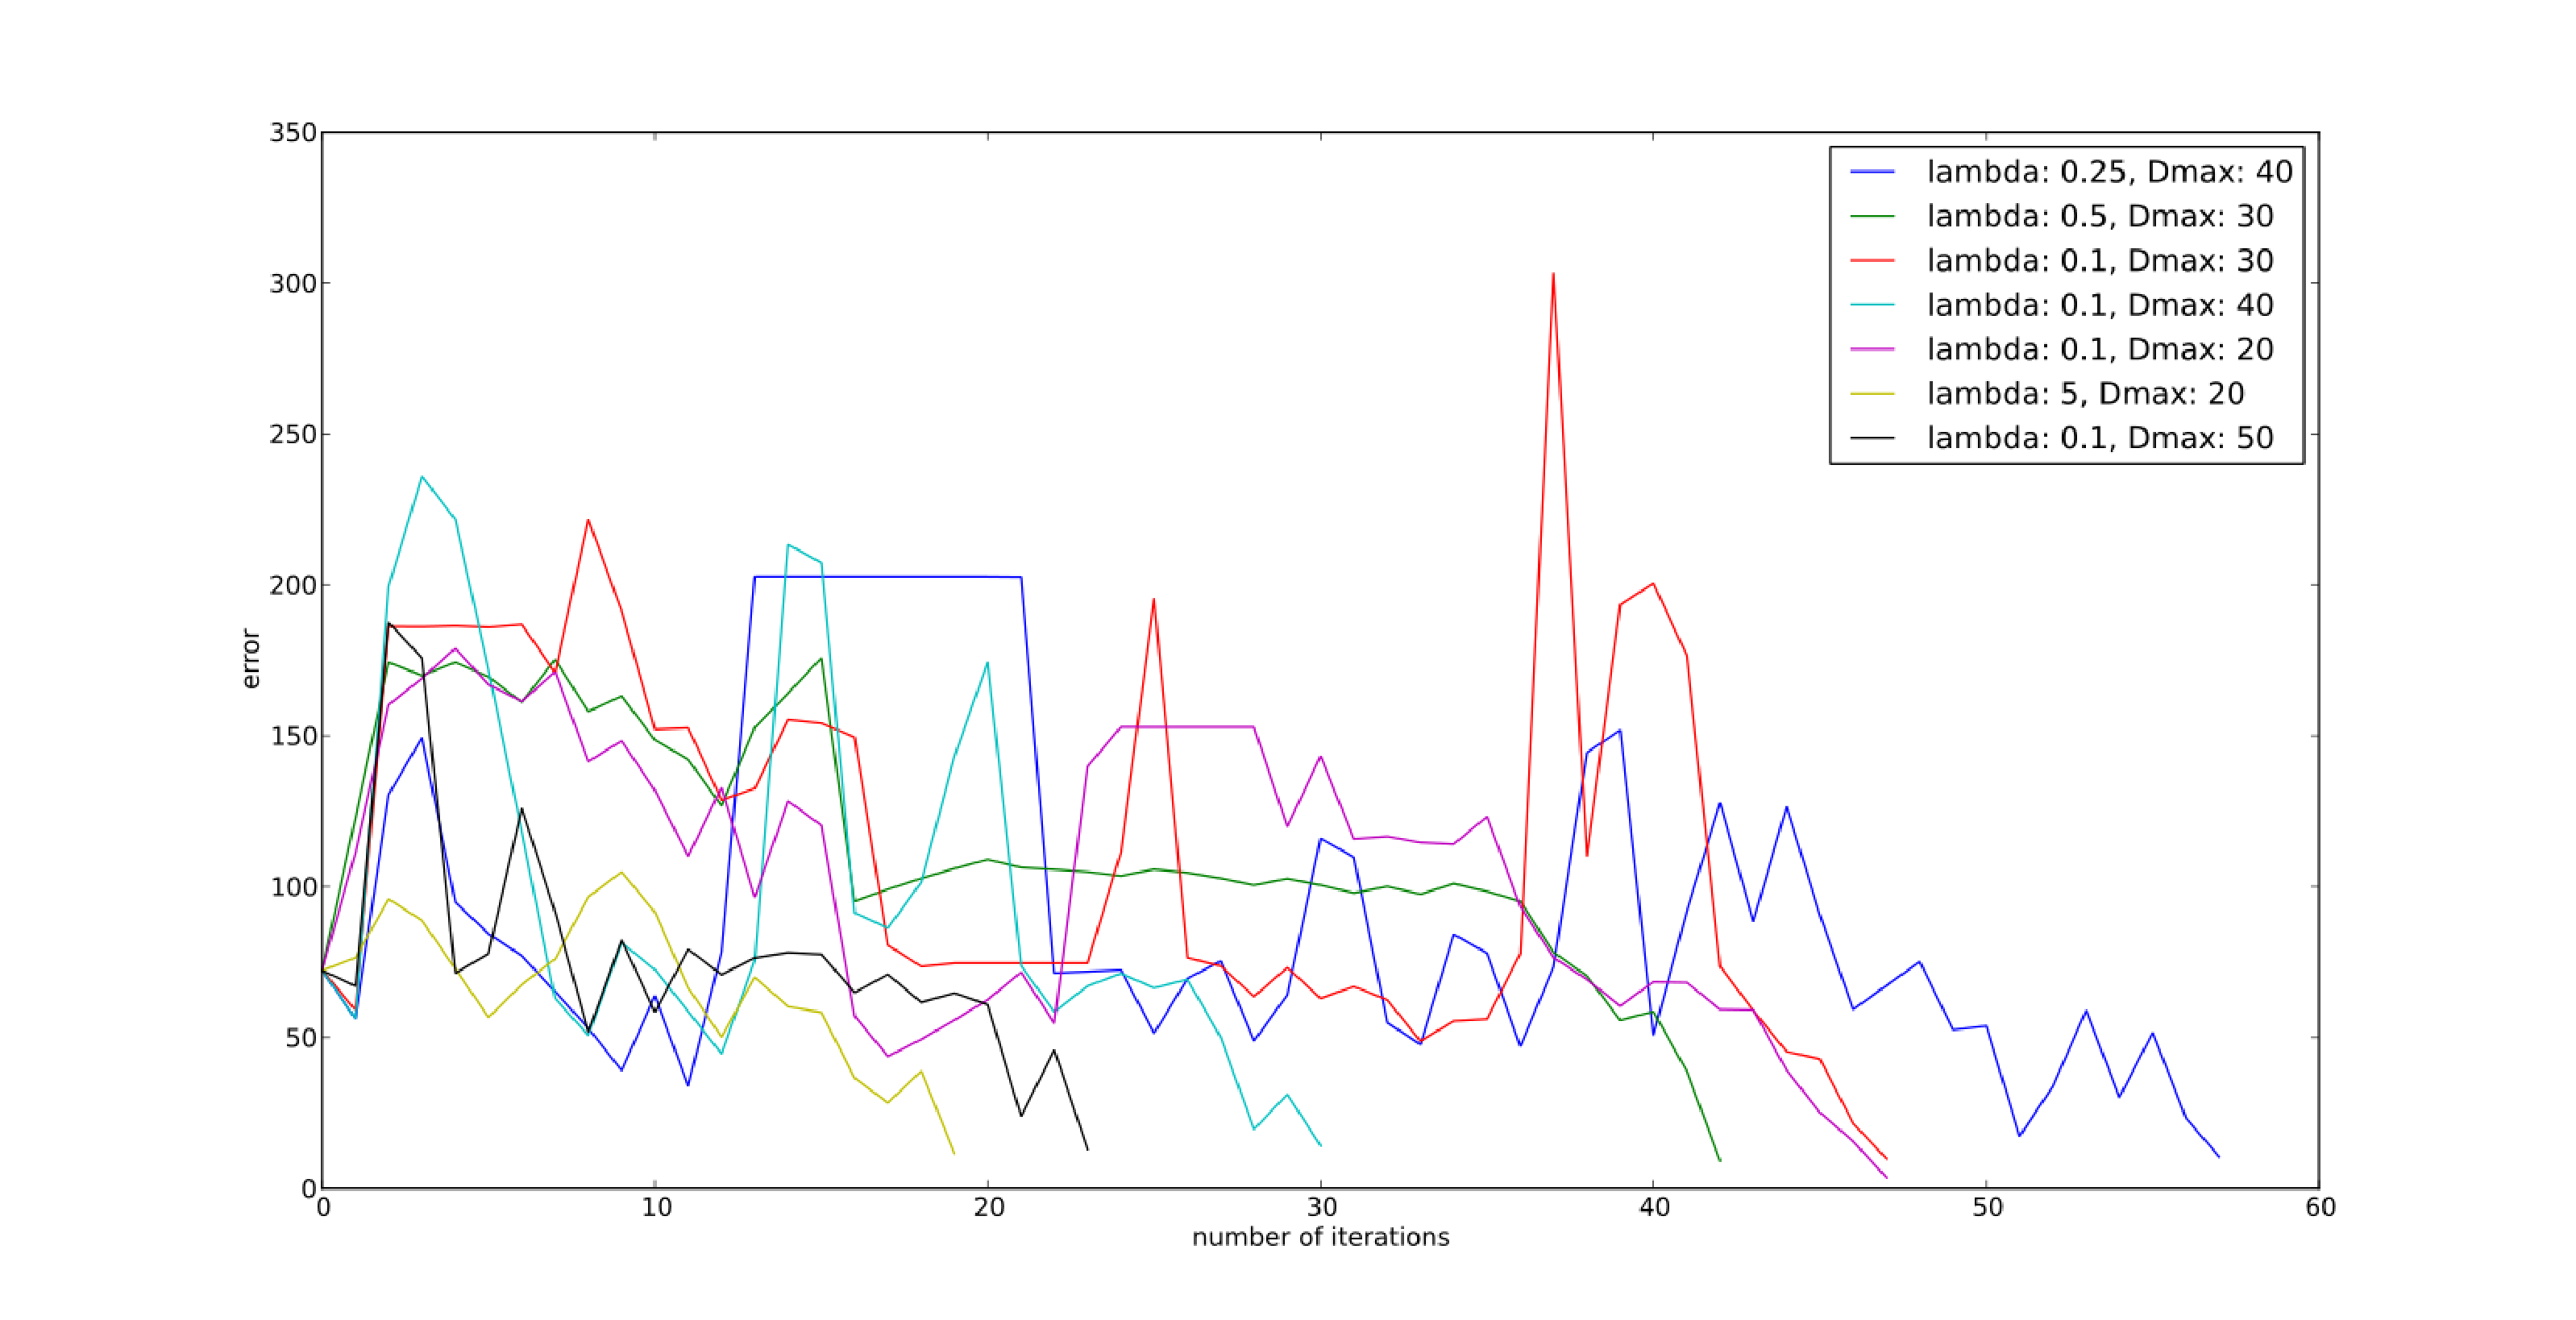
\includegraphics[width=1.3\textwidth]{pics/ik_3.pdf}
  }
  \caption{The third position, with the positional error set out against
         the time.}
  \label{fig:ik_plot3}
\end{figure}
\FloatBarrier

In each case, the optimal value for $\lambda$ was 5, while $D_{max}$ was either
50 or 20, which is a relatively large difference given the range of values. Of
course, three tests isn't enough to conclusively determine the optimal
parameters, but they offer a nice starting point for further practical testing.


\subsection{Calculating the retraction point}
\begin{figure}[htbp]
  \centering
  \makebox[\textwidth] {
    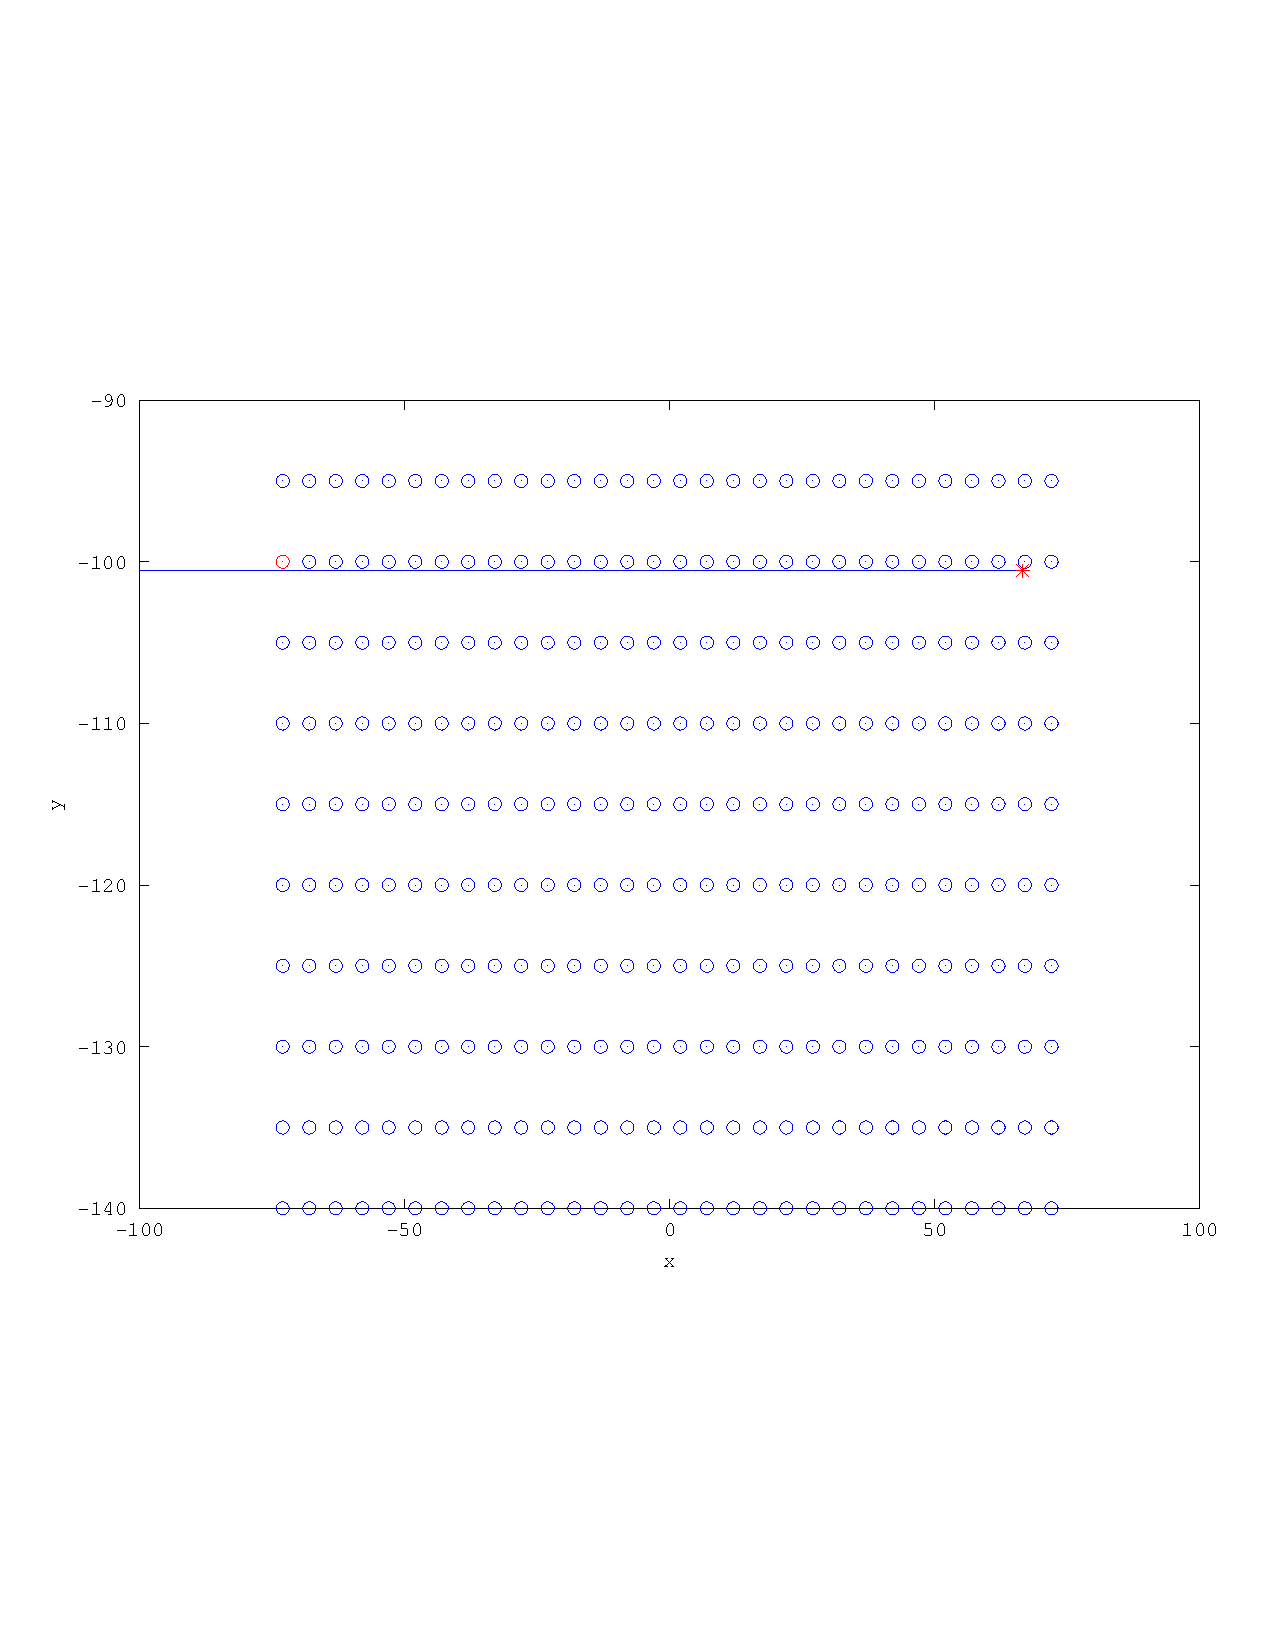
\includegraphics[width=0.8\textwidth]{pics/retract.pdf}
  }
  \caption{Visualistation of relevance of all tried retraction points. The red
      point is the finally used point. The red asterisk is the contact point. In
      tis case the ball should be kicked straight forward.
         }
  \label{fig:retraction_plot1}
\end{figure}
\FloatBarrier
To see how well the calculation of the retraction point really works, we
visualised the different points that were tried out. Figure \ref{fig:retraction_plot1}
is the result of a direction 
$\begin{bmatrix} 1 \\  0 \\ 0 \end{bmatrix}$ and a center of mass positioning of
    the ball right in front of the right foot (the kick commenced with the right
    leg as well). The line is the point on which we
    would like to see the foot retraction take place, as it is the line on which
    both the direction and the contact point of the ball lie. The blue dots are
    the reachable positions that are evaluated as possible retraction points. The red dot is the
    chosen retraction point the Nao executes, and the red asterisk is the contact
    point. For this experiment we chose 
    $\delta = 0.999$ in equation \ref{eq:delta}, so that accuracy was more important than distance. The
    effect is in this case that still the point with the greatest distance is
    chosen because the whole row of those points have the same accuracy so still
    the one with the biggest distance to the contact point gets chosen.

Another experiment shows the same idea but, instead of kicking straight ahead,
the direction was with an angle to the left, more precise with  $\vec{e} =
\begin{bmatrix} \frac{1}{\sqrt{2}}\\
\frac{1}{\sqrt{2}} \\ 0 \end{bmatrix}$. Using the same $\delta$ value as before gave us
the result as can be seen in figure \ref{fig:retraction_plot2}. It is the most
accurate point given a list of possible elements. 

Although there is another good point (at approximate (-60, -140)) it is nearly
impossbile to get this value as the chosen optimal point. When lowering the
$\delta$ value even slightly it changes the distance drastically in the x
direction, making the trade-off less pronounced than imagined.

\begin{figure}[htbp]
  \centering
  \makebox[\textwidth] {
    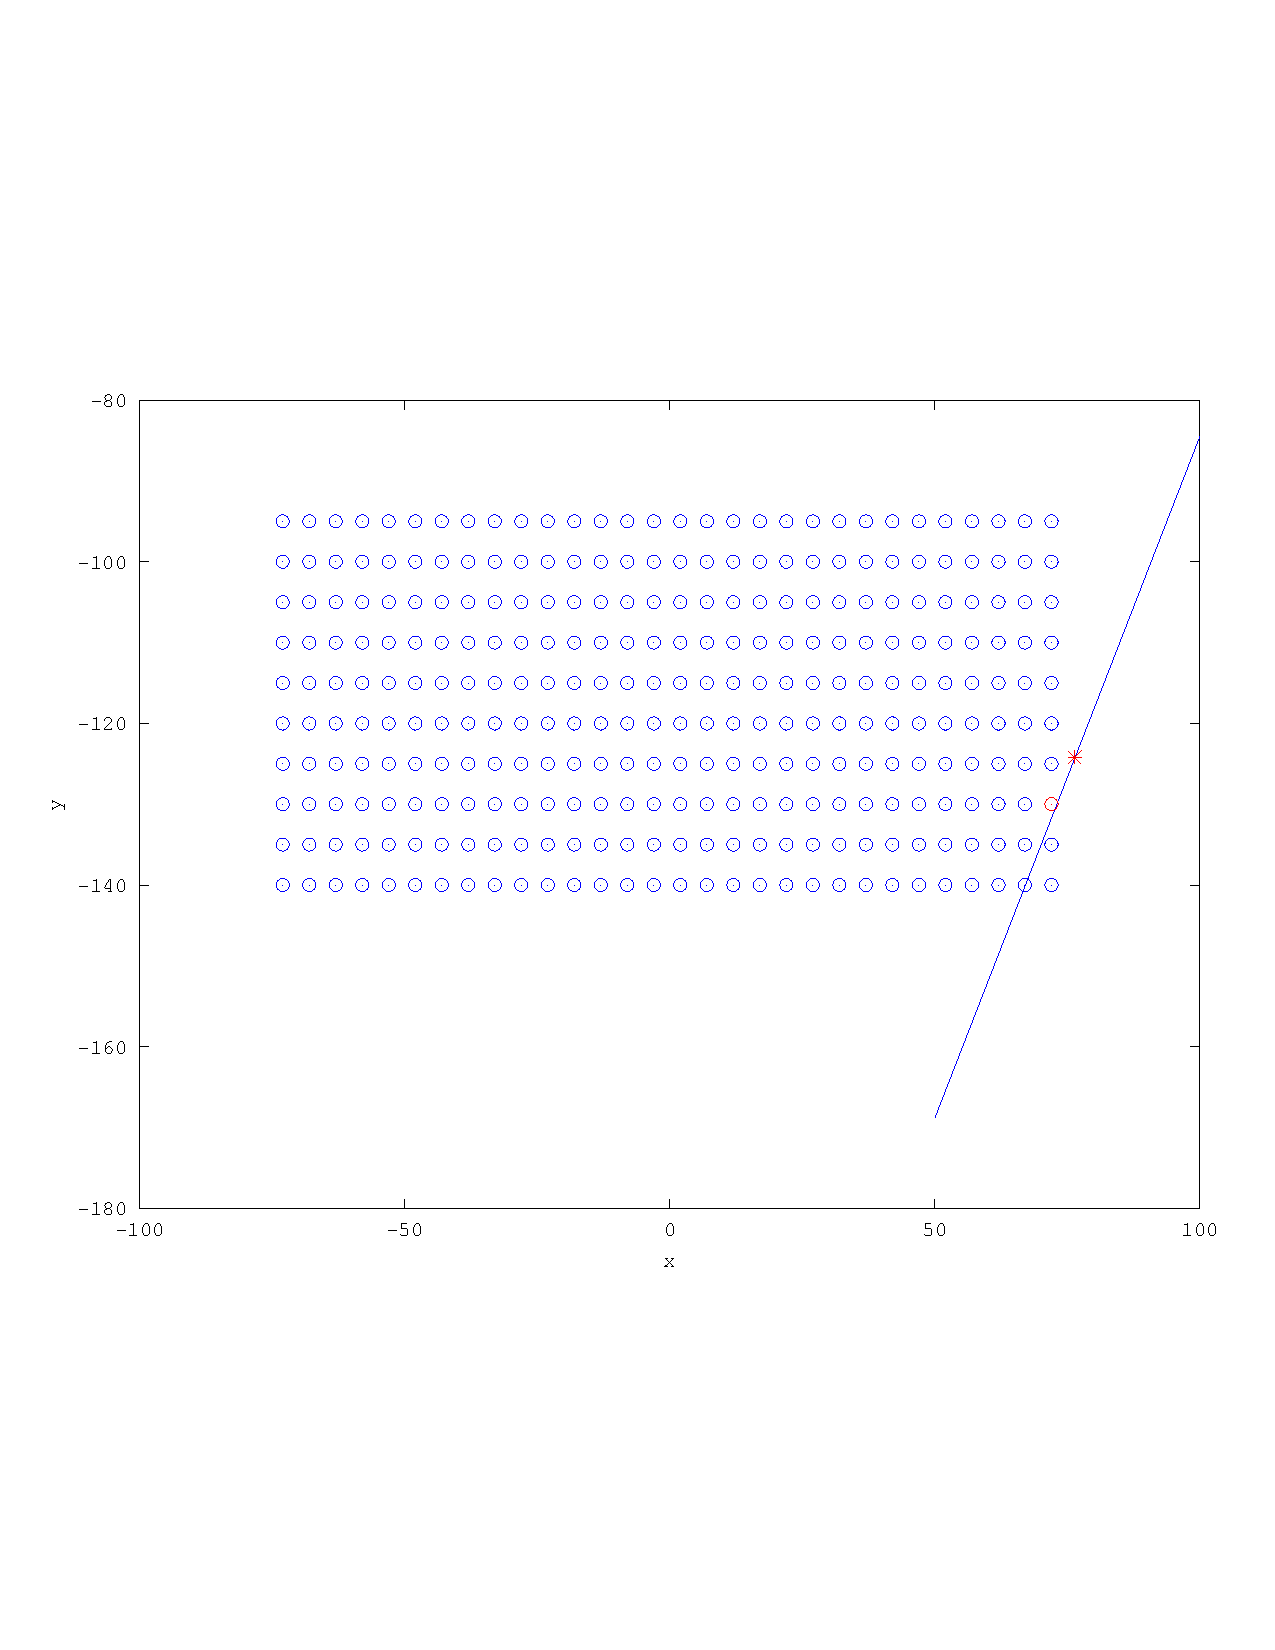
\includegraphics[width=0.8\textwidth]{pics/retract3.pdf}
  }
  \caption{Visualistation of relevance of all tried retraction points. The red
      point is the finally used point, the red asterisk is the contact point. 
      In this case the ball is kicked with an angle.
         }
  \label{fig:retraction_plot2}
\end{figure}

Another visualisation can be seen in figure \ref{fig:retraction_plot3}. In this
case the ball should be kicked straight ahead again ( direction = $\begin{bmatrix} 1 \\  0 \\ 0 \end{bmatrix}$). All blue dots are evaluated retraction points and the red stars are the points that are the most
accurate(all have the same value). The data is set out over the $xy$ axis, which
is the added length of the $x$ and $y$ direction, the $z$ axis and the
$distance$ is the distance as we measure it in \ref{eq:distance} between contact point and the ball. The fact that sometimes multiple of the same $xy$ and $z$
combinations have different distances to the contact point is to be understood from
the fact that although in the axis both the real value of $x$ and $y$ are added to
eachother, equation \ref{eq:distance} only considers the value of $x$ when the ball should go
straight ahead.

\begin{figure}[htbp]
  \centering
  \makebox[\textwidth] {
    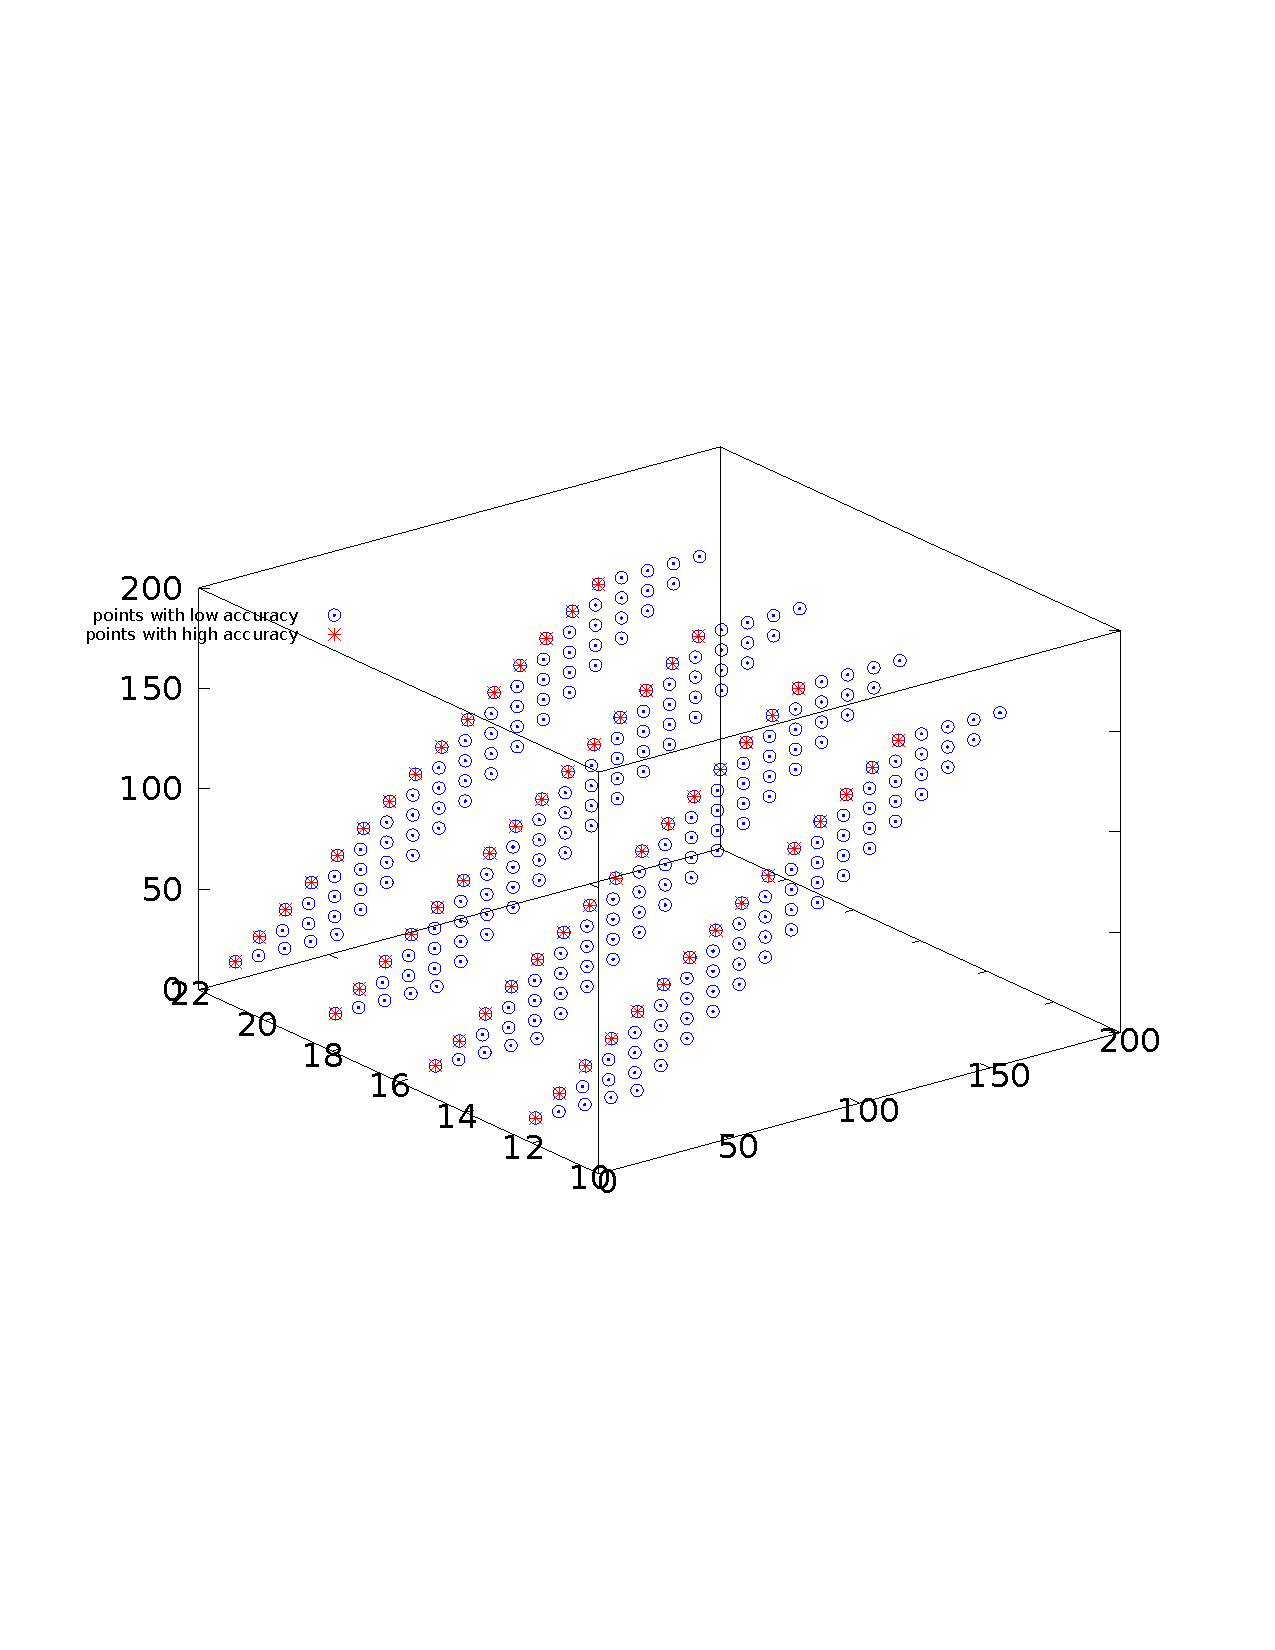
\includegraphics[width=0.8\textwidth]{pics/uglyplot.pdf}
  }
  \caption{Plot where the length of the $xy$ direction between the contact point
      and the retraction point are set out against the $z$ direction and the $
      distance$ from equation \ref{eq:distance}. The red points indicate the
      most accurate position
         }
  \label{fig:retraction_plot3}
\end{figure}

\FloatBarrier

\subsection{Integration of the Center of Mass balancers with the kick}
Because of the limited ranges of both legs when it comes to reaching a ball we
would like the Nao to stand straight as much as possible while performing a kick. 
When executing the initial pose we use the CoM balancer to seek the most
balanced position, but it makes a lot of difference as to which joints in the
support leg are used for balance. At first we experimented  with the
\emph{HipRoll} and \emph{HipPitch} to move to the most stable position. This
however made for quite an unnatural pose, as you can see in Figure
\ref{fig:subfig1}. Because executing a kick only uses the kicking leg, it can
reach less of the relevant places. 

\begin{figure}[ht]
\centering

\subfigure[Using the \emph{HipRoll} and \emph{HipPitch} to balance the Nao]{
   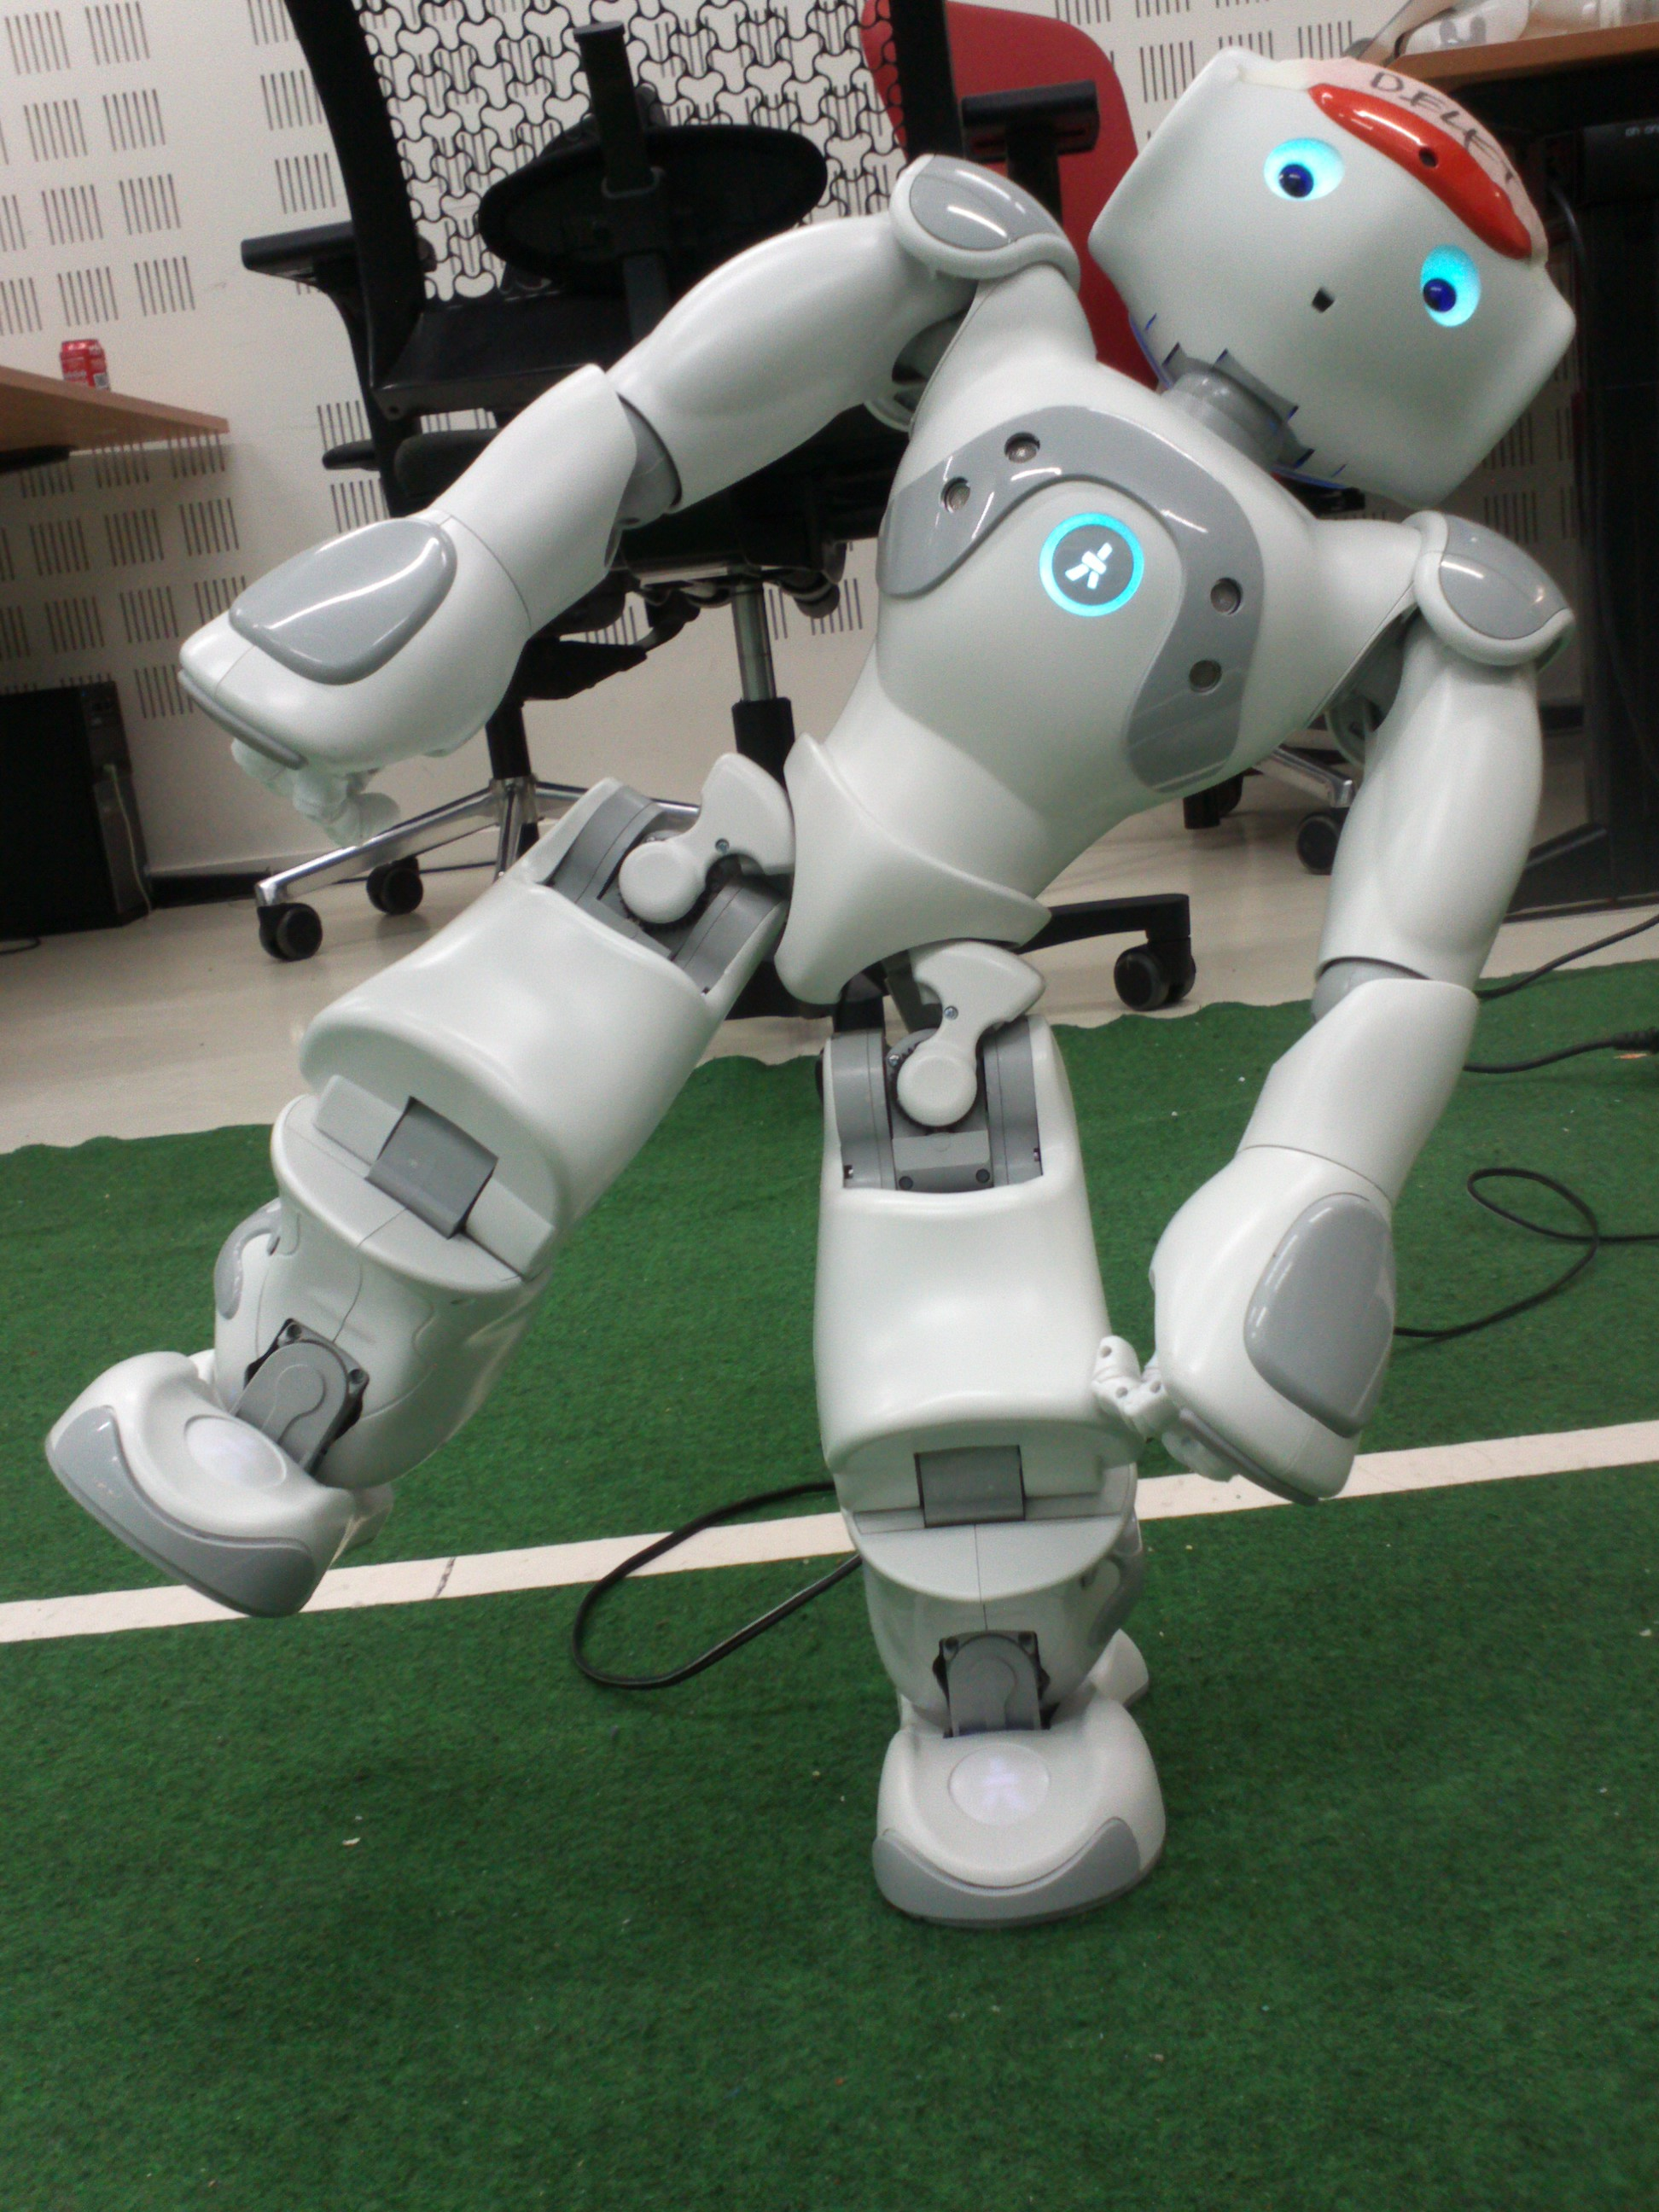
\includegraphics[width = 0.4 \textwidth] {pics/nao_initial1.jpg}
   \label{fig:subfig1}
 }

 \subfigure[Using the \emph{AnklePitch} and \emph{AnkleRoll} to balance the Nao]{
   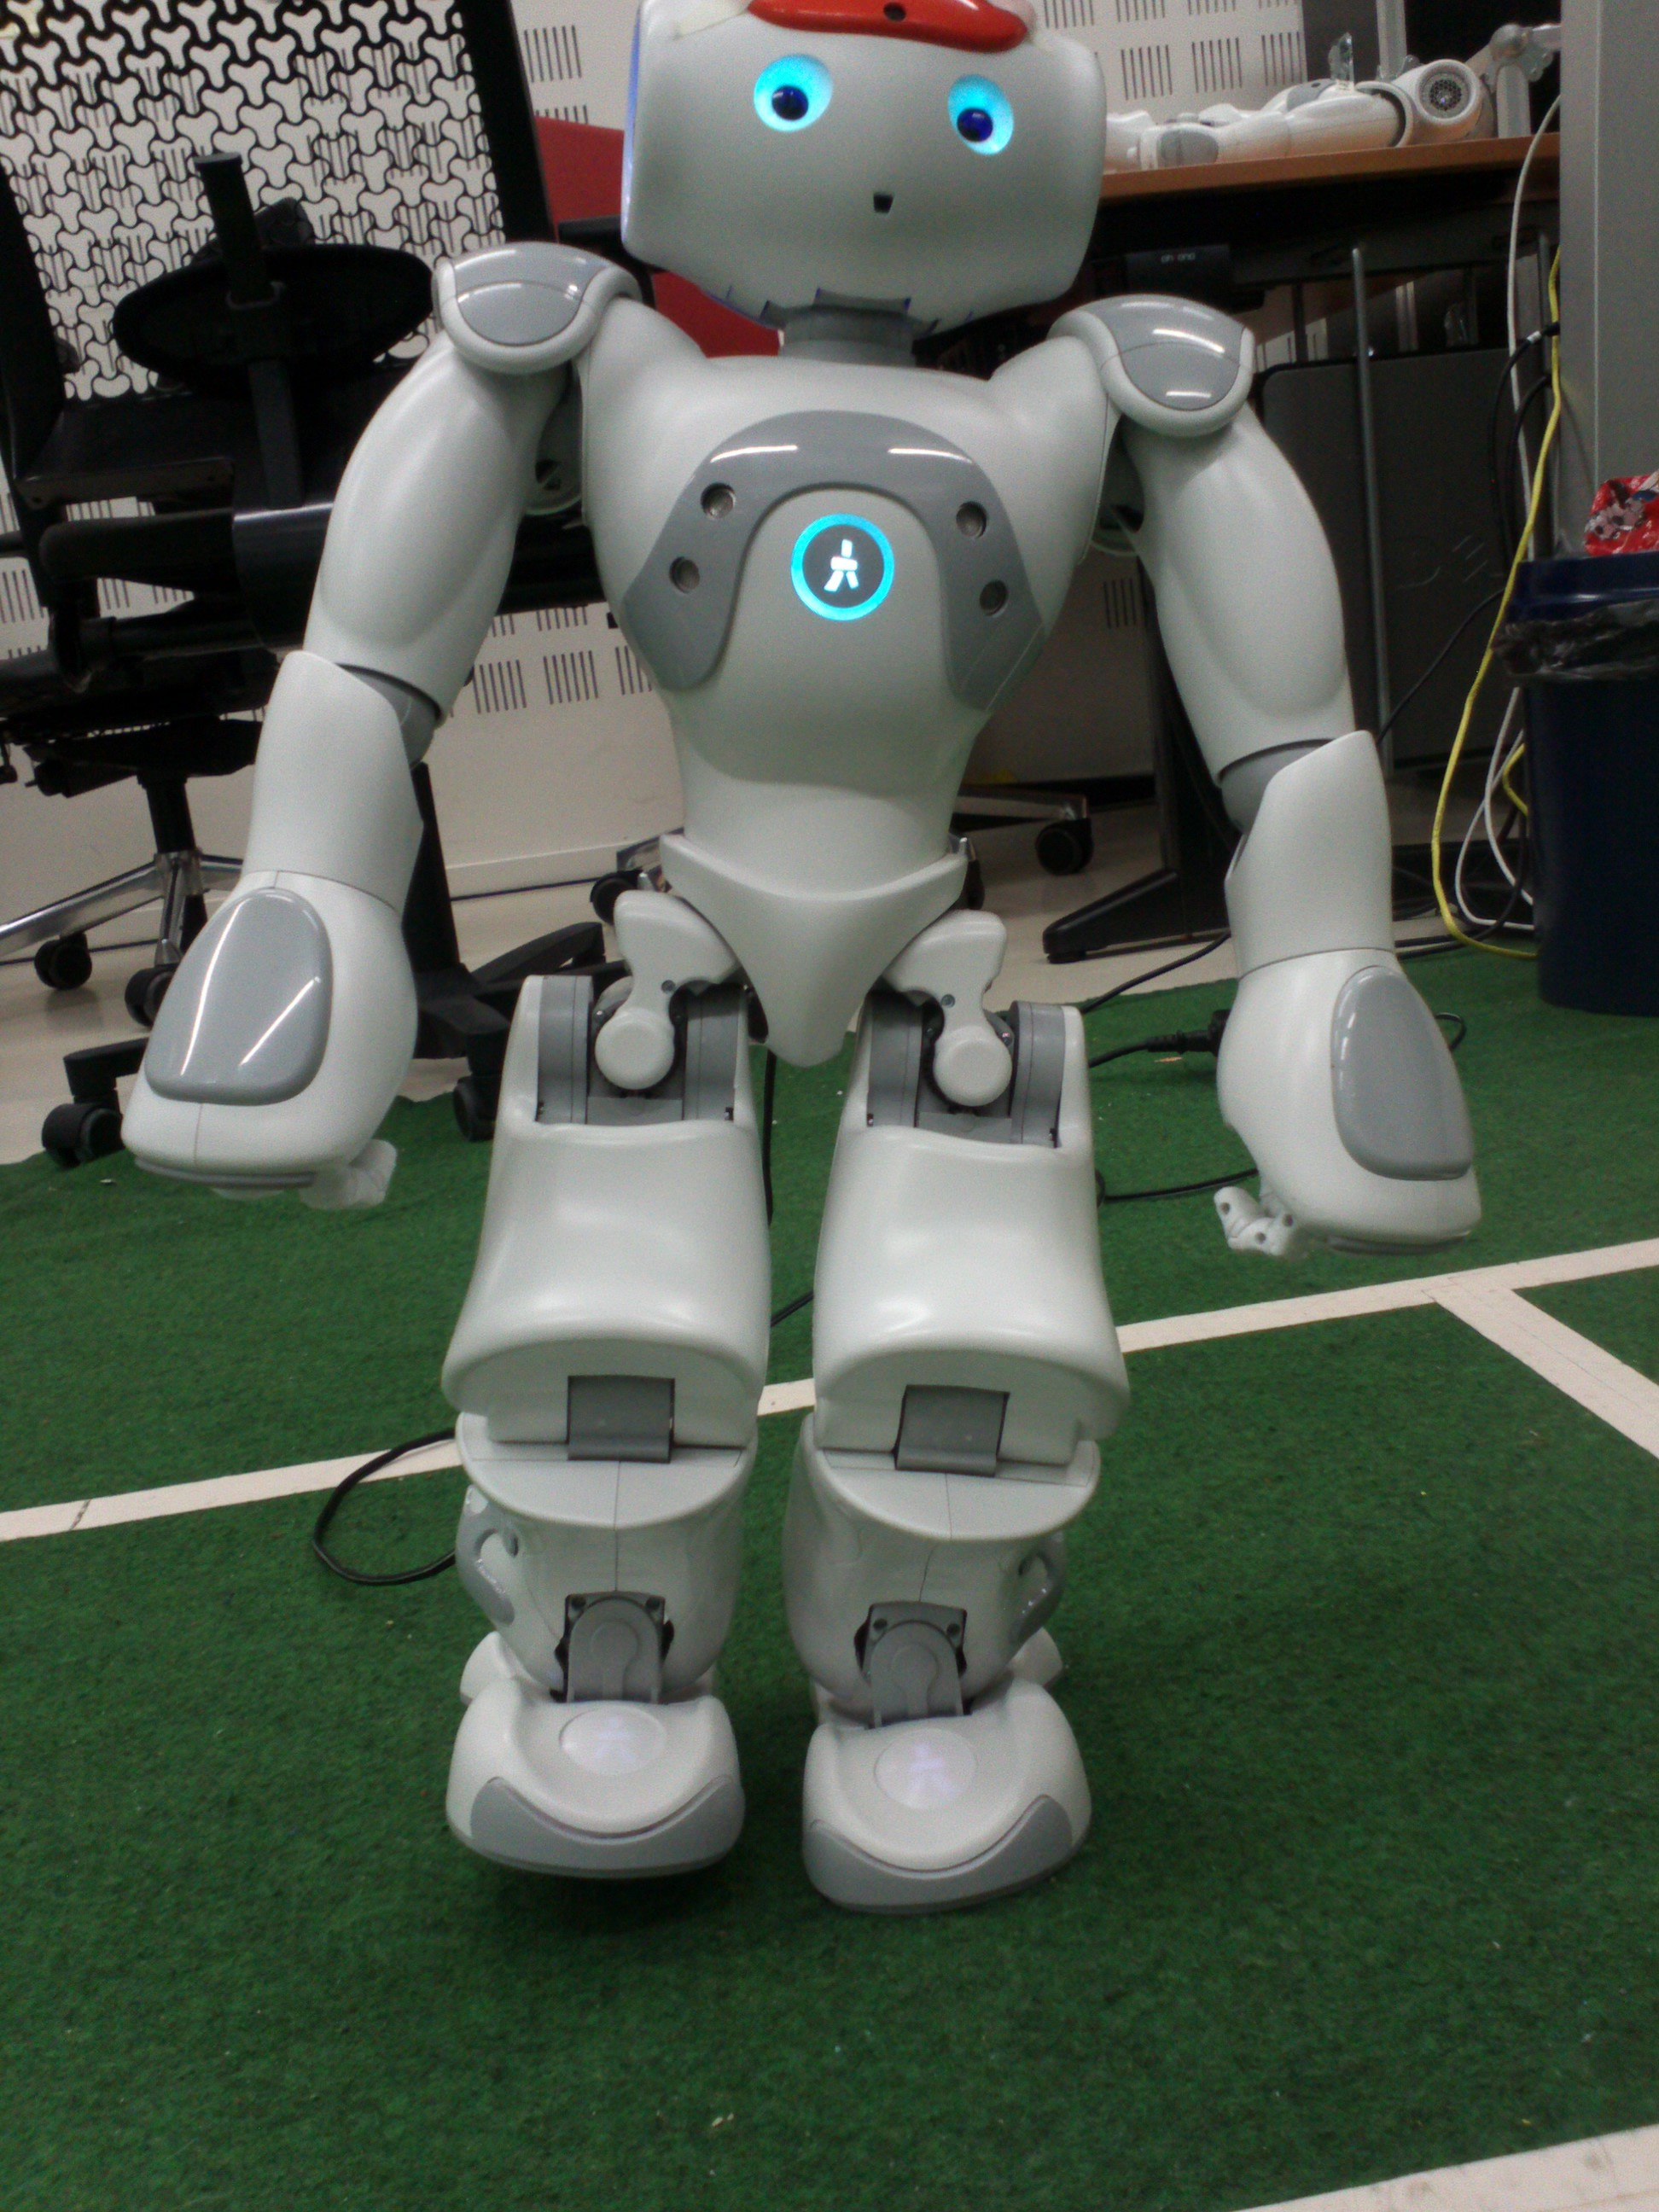
\includegraphics[width = 0.4 \textwidth] {pics/nao_initial2.jpg}
   \label{fig:subfig2}
 }

\label{myfigure}
\caption{Experimentation with the influence of joint choice on the balancer}
\end{figure}
Using the angle of the \emph{AnkleRoll} and \emph{AnklePitch} in the initial
pose delivers a more natural position as seen in Figure \ref{fig:subfig2},
which makes it a better deicision for the initial pose. 

\section{Conclusion}
Although the individual components mostly work as planned, integrating
them all into an actual kick has proven harder than expected, which
has left us unable to test the interactions between all of the
components. For instance, using only the hip to compensate for balance
is effective in the sense that it's good at balancing, but it results
in poses where the kicking leg is unable to reach even near the
ground. Using the ankle however works just as well for balance, and
doesn't suffer from the same problem. Unfortunately, there was no time
for further testing in this regard.

Generation of the kick trajectory appears to work properly, although it hasn't
been thoroughly tested (only in a few directions) due to time
contraints. Similarly, there is no data regarding the strength or stability of
the kick, simply because there is no final kick yet.

The balancing system seems to work quite well and has been quite vigorously
tested. Still interferences from the side stay problematic, but only playing a
real math with the balancing turned on will show if it will work decent enough.

In the end, we've ended up with a nice motion framework which needs a bit more
work in order to have a completely functioning kick, which will hopefully function
as a basis for further motion-related tasks for the Dutch Nao Team (such as a
new walking motion).

\subsection{The retractionpoint} 
The above experimentations with finding a retractionpoint while making
a trade-off between accuracy and distance seems to conclude that the
retraction calculation works as was expected for the basic cases. Due
to time constraints, and the fact that less straightforward kicks are
hard to visualise on a graph there are still cases left out, but it
already makes for a succesful kick in the most basic of situations.

\section{Discussion}
Although the problem of making a dynamic kick has been solved by various teams
in the Standard Platform League already (citations, citations), there are various solutions to our
problems that we have not yet encountered in other papers. For instance the idea
of making a proportinal controller based on the Center of Mass is one that is
implemeneted often, but making a search space through which to find the optimal
position is not one we have encountered but works great.

It comes to show that although our problem initially looked as if it would be a
straight path we have been able to give it our own interpretation which only
gives the 

\section{Future works}
Now that all sub problems of making a dynamic kick seem to be solved succesfully, there are still some future improvements we would like to work on.

\subsection{Wrapping up our current work}
Firstly, we would like to integrate all elements talked about to make a succesful kick. This
was something we wanted to complete by the time this project ended, but in
hindsight was a little too advanced for the limited
timeframe. Nevertheless, we were still  able to find
solutions to every problem and can take our time to combine both controllers
and the kicking motion into a worthy final result.

\subsection{Porting everything to C++}
Many components were written in Python to aid in rapid prototyping, with help
from the Numpy module to allow for acceptable speeds. This works decently, but
we unfortunately don't have a way of running Numpy on our robots. Seeing as the
Dutch Nao Team plans on switching to C++ for their codebase in the near future,
porting everything to C++ seems like the best option.

\appendix
\section{Experimentations with solving the inverse kinematics problem.}
\label{A}
Before we arrived at our final inverse kinematics solution, we tried a number of
different (seemingly easier) options first.  This section details some of these
experimentations and why we have abandoned them.

\subsection{Using built-in functions}
The Naoqi framework running on the Nao robots offers a \emph{Cartesion Control
API}\footnote{http://www.aldebaran-robotics.com/documentation/naoqi/motion/control-cartesian.html}
which contains a number of inverse kinematics function for setting and
requesting end effector locations in a specified coordinate system.  The
possible coordinate systems were ``world'' (where the origin was somewhere
arbitrarily around the Nao), the torso and one between the legs. Because both
the torso coordinate system and the one between the legs are dependent of the
posture of the Nao , we tried to work with the coordinate somewhere in space.
To determine the range of the legs we took the Nao by hand and set the legs in
the most stretched positions and retrieved the maximum
and minimum $x$ ,$y$ and $z$ values.  These were taken as absolute ranges
relative to a starting position. In the end this approach
didn't work as making a request for the current position as well as setting a
new position in this coordinate frame was not reliable enough. It seemed that
the sensor values used to find these positions weren't well enough to use for
such an operation. Another big problem is that actuation appeared to be quite
slow; far too slow for a powerful football kick.

\subsection{Using a simulator to find all reachable positions}
We also tried to use the Cartesion Control API in
a simulated environment\footnote{The environment used can be found on
http://www.nao.sandern.com} to obtain a table containing all reachable locations
of a given leg, within a certain resolution.
Throughout a given range of world positions, the Nao was made to move its foot
there, after which the position of the foot was requested to see if the position
had been reaches.
In the end this was not as reliable as hoped due to the same issues as spoken in
the last section.

\subsection{Making a lookup-table using Forward Kinematics}
Because we already had a workable solution for forward kinematics, we thought
about creating a lookup table by iterating through a collection of joint angles
and saving them in a hashmap along with the corresponding end effector position.
Integrating this using the balancing system however became a bit harder because
we needed to track the position of the hip angles (these were, at the time used
for changing the pose of the Nao) in the support leg, and in the end
constructing the inverse kinematics ourselves was an easier solution.

\bibliographystyle{plain}
\bibliography{library}
\end{document}
